\section{Two-dimensional bump-in-channel}
Upon completion of the validation of the flow over a flat-plate, the turbulent flow on a two-dimensional bump-in-channel case was investigated. This case is also available on~\cite{tmr} under the name ``2D Bump-in-channel''. This case was only run with syn3D.

The problem domain and flow conditions are shown in~\Cref{fig:2dbump}. It is referred to as two-dimensional due to the shape of the bump not depending upon the $z$ coordinate, as opposed to the three-dimensional bump in~\Cref{sec:syn3dbump}.

This case is different from the previous flat plate case because it involves wall curvature, which induces a pressure gradient. The TMR website also provides five grids for this case.
\begin{figure}
    \centering
    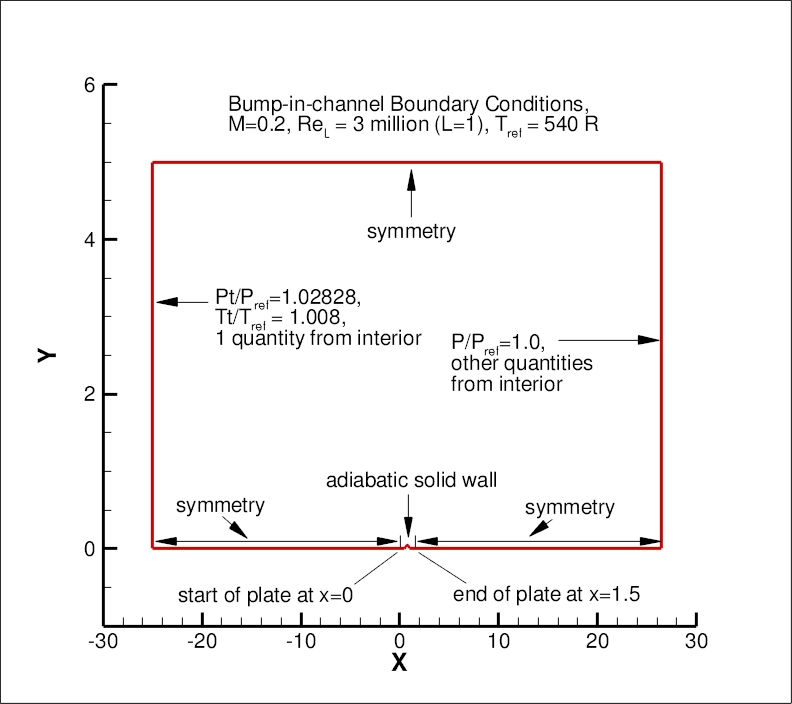
\includegraphics[width=0.7\textwidth]{figs/2dbump/bumpBCpic.jpg}
    \caption{Turbulent two-dimensional bump case~\cite{tmr}.}
    \label{fig:2dbump}
\end{figure}

\begin{table}[ht!]
    \centering
    \caption{2D Bump (syn3D): Comparison of force coefficients for the finest two-dimensional bump.}
\label{tab:syn2dbump1}
\begin{tabular}{@{}lcccc@{}}
\toprule
Solver & $C_L$ & $C_D$ & $C_{Dv}$ & $C_{Dp}$ \\
\midrule
CFL3D & 0.0249 & 0.0036  & 0.0032 & 0.0004  \\
syn3D & 0.0251 &  0.0035 & 0.0031 & 0.0004  \\  \bottomrule
\end{tabular}

\end{table}

\begin{table}[ht!]
\centering
\caption{2D Bump (syn3D): Comparison of skin friction coefficient at various locations.}
\label{tab:syn2dbump2}
\begin{tabular}{lccc}
\toprule
& \multicolumn{3}{c}{$C_f$} \\
\cline{2-4}
Solver & $x=0.75$ & $x=0.6321975$ & $x=0.8678025$ \\
\midrule
CFL3D & 0.00615 & 0.00519  & 0.002680   \\
syn3D & 0.00610 & 0.00519  & 0.002835  \\
\bottomrule
\end{tabular}

\end{table}

\Cref{tab:syn2dbump1} tabulates the drag coefficient, the lift coefficient $C_L$ as well as the contributors to the drag coefficient $C_{Dv}$ and $C_{Dp}$, which represent the contributions due to viscous forces and pressure forces respectively. \Cref{tab:syn2dbump2} tabulates the skin friction coefficient probed at various locations. These tables show good agreement between CFL3D and syn3D.

\Cref{fig:syn2dbumpcnvstudy} shows the convergence for all grids. Reduction of the residual is quite slow for this particular problem, with the finest grid taking over 3 days on 64 processors to complete. In addition, a plateau of the residual at approximately $2\times10^{-3}$ can be observed for the three coarsest grids, which is likely due to the interfaces between the symmetry planes and the solid wall. In fact, the maximum residual occurs at the field points with faces lying on that interface, which is also an interface between block boundaries.
\begin{figure}[ht!]
\centering
\begin{subfigure}{.7\textwidth}
  \centering
  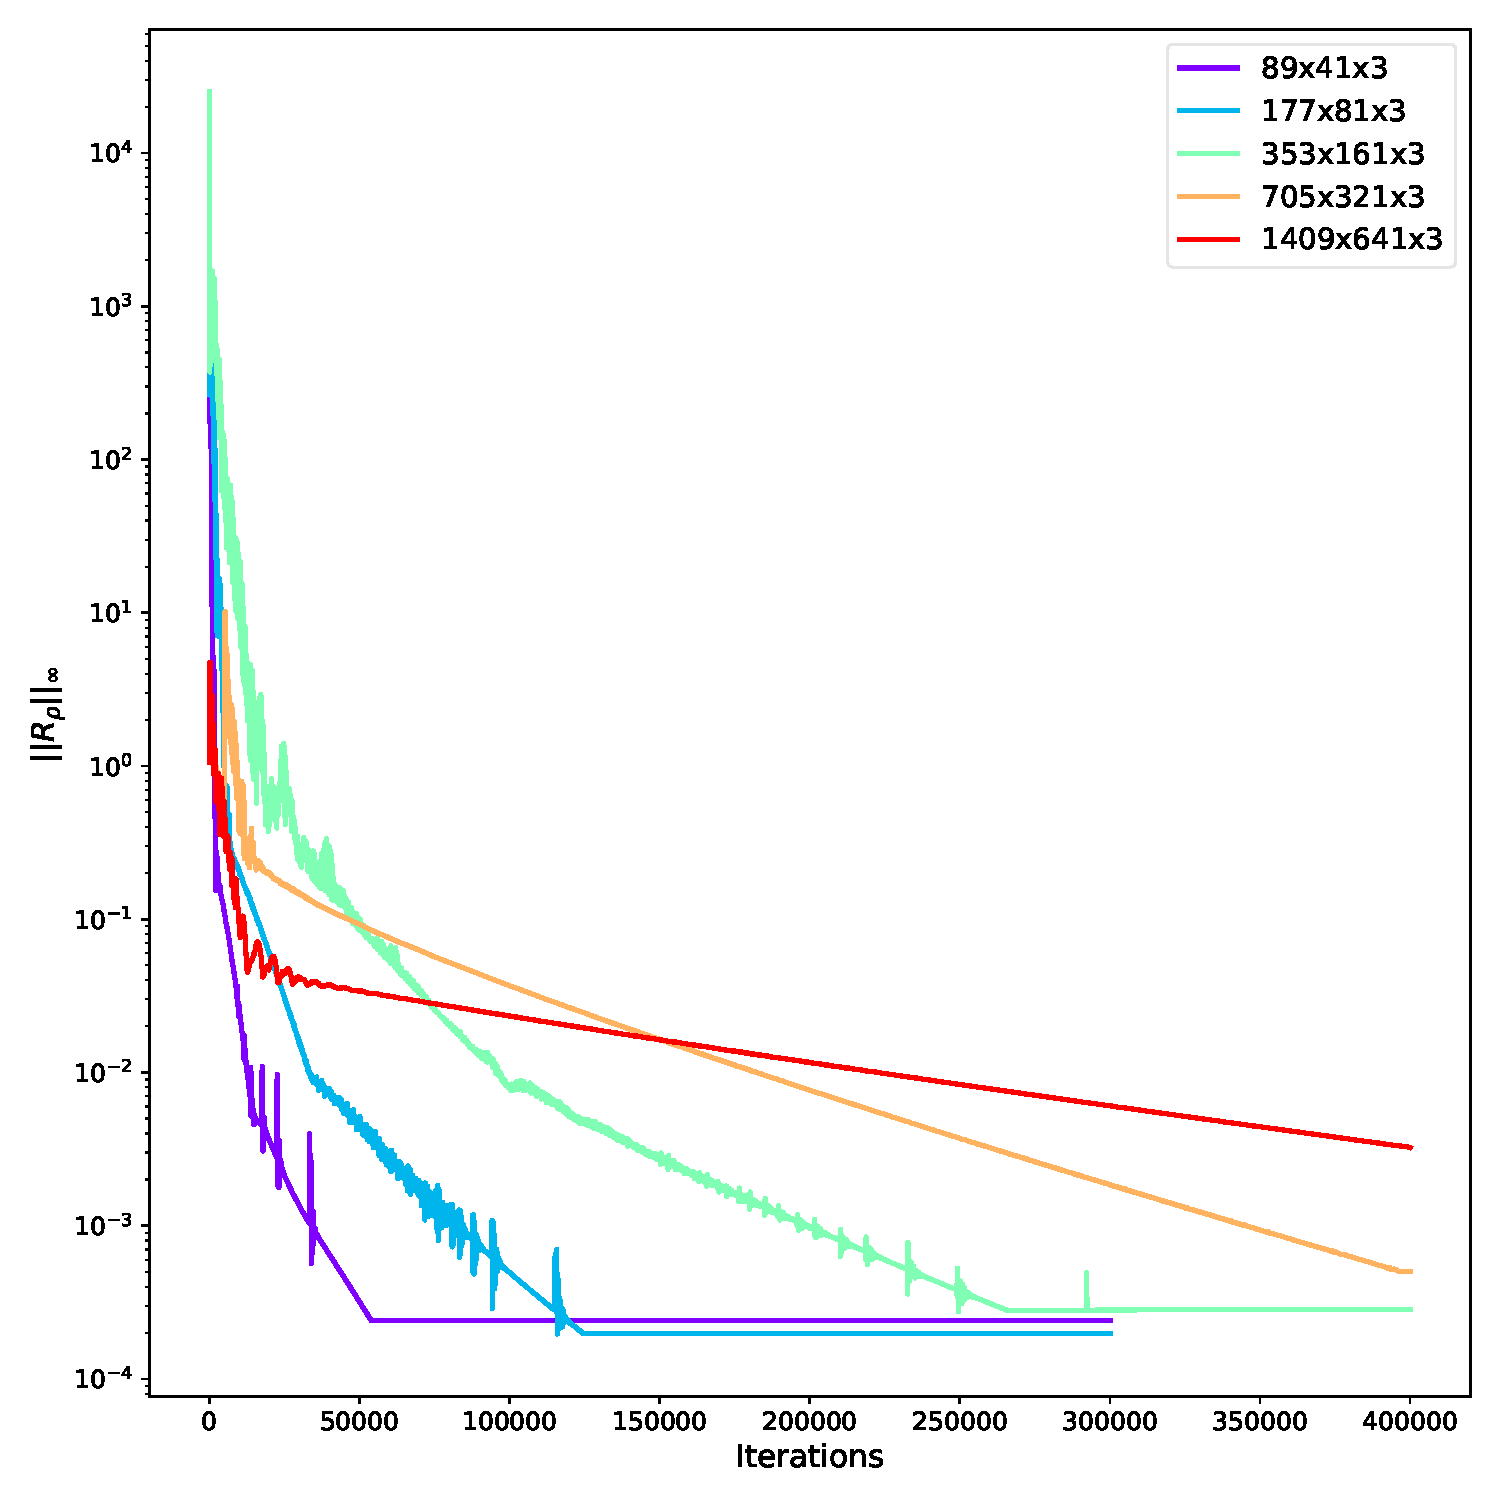
\includegraphics[width=1.0\textwidth]{figs/2dbump/convergenceRho.pdf}
  %\caption{Maximum density residual}
\end{subfigure}%
%\begin{subfigure}{.45\textwidth}
%  \centering
%  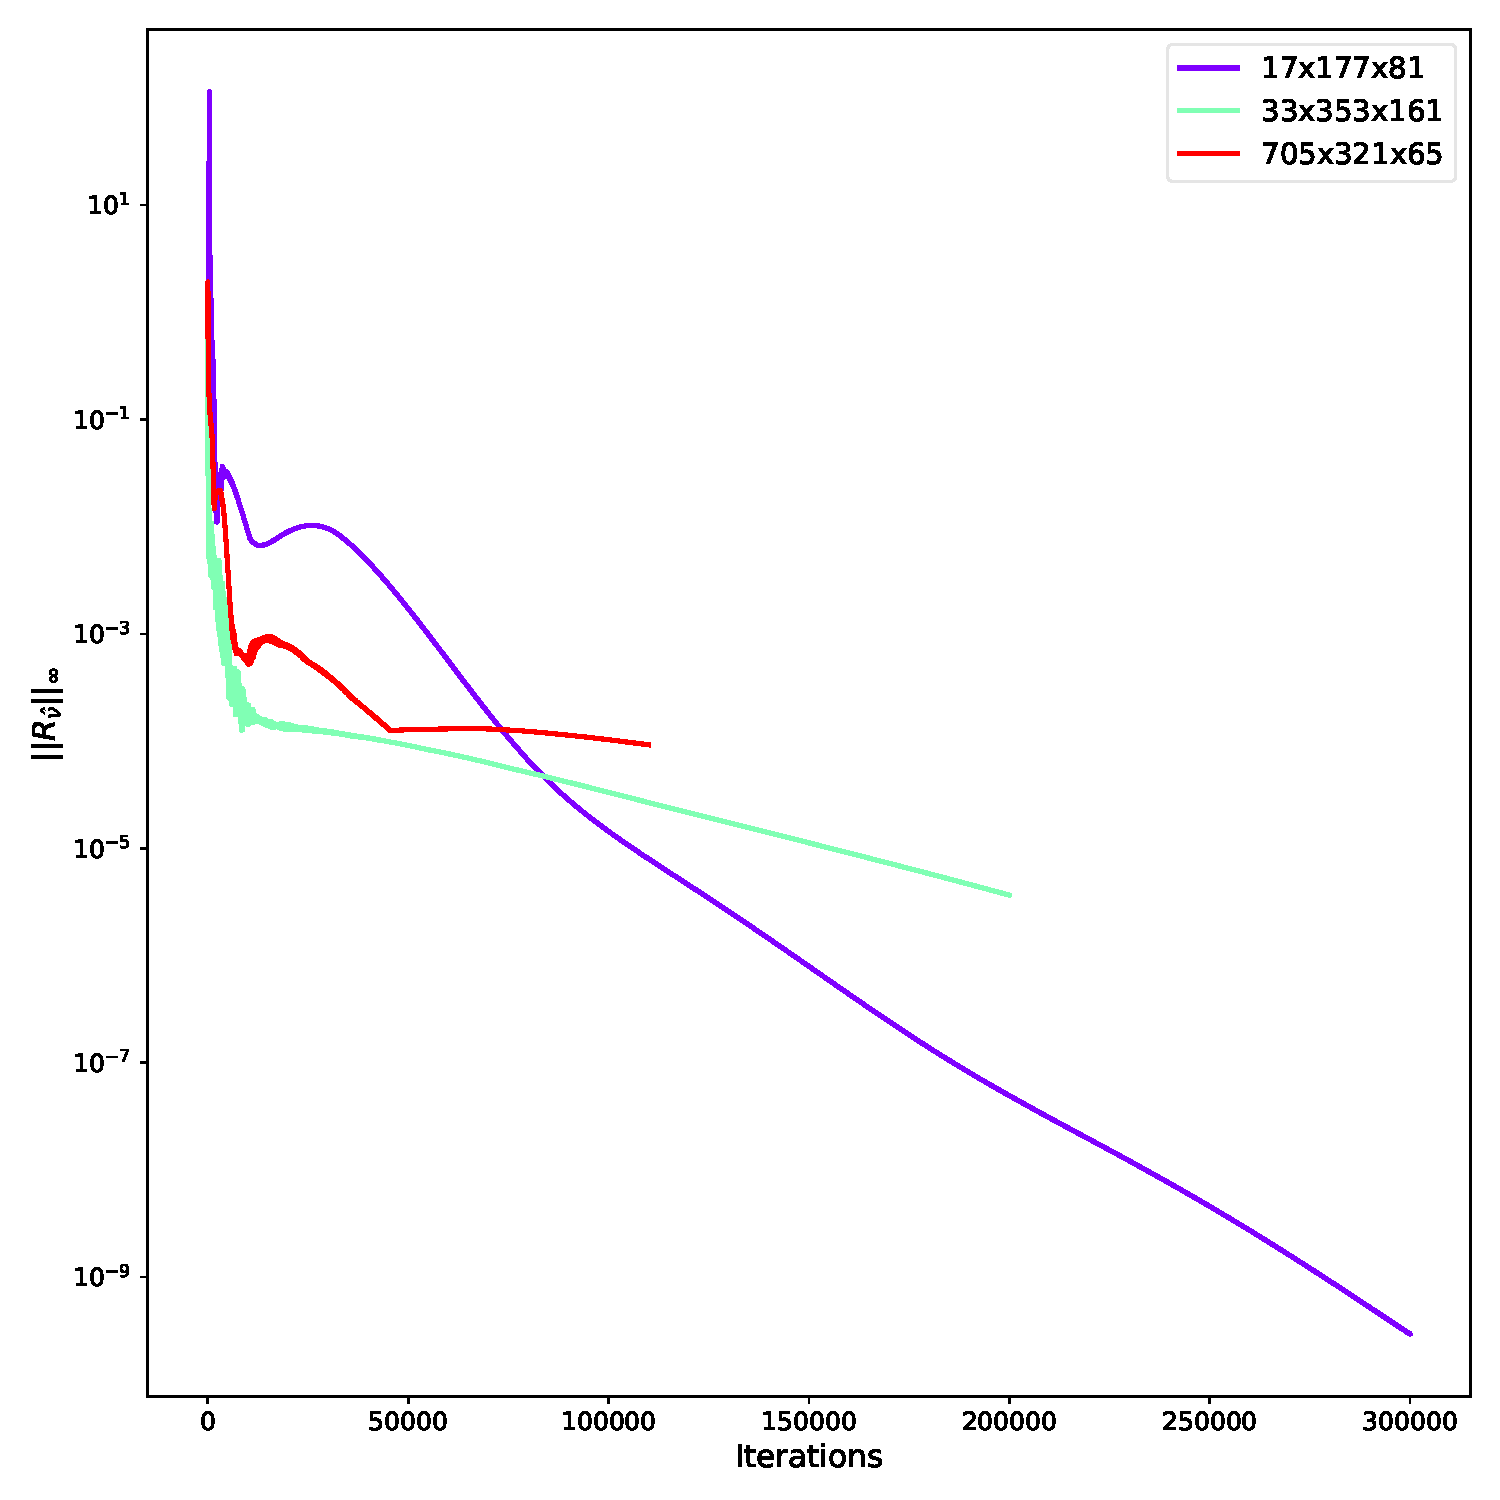
\includegraphics[width=1.0\textwidth]{figs/2dbump/convergencesa.pdf}
%  \caption{Maximum turbulence variable residual.}
%\end{subfigure}
\caption{2D Bump (syn3D): Convergence of maximum density residual on various grid sizes.}
\label{fig:syn2dbumpcnvstudy}
\end{figure}

\begin{figure}[ht!]
\centering
	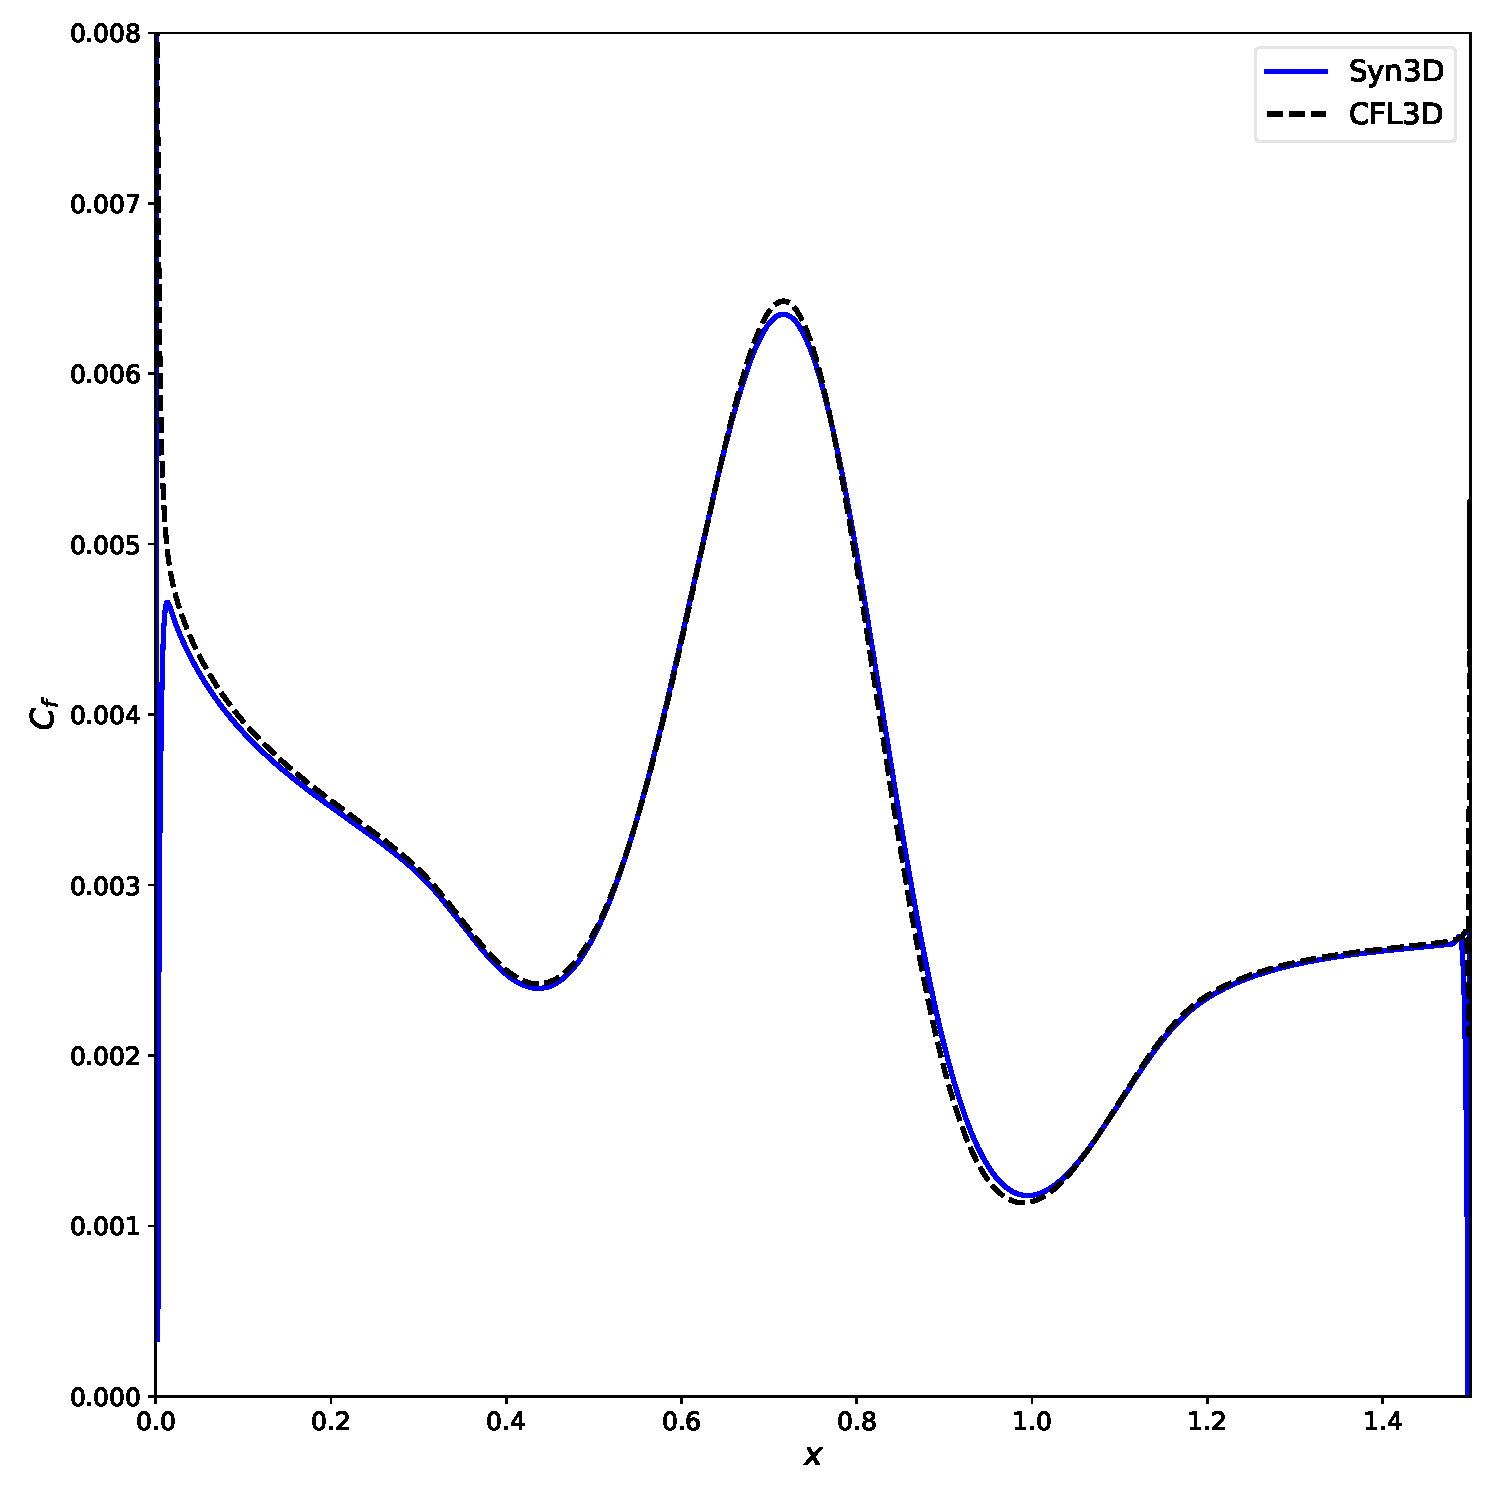
\includegraphics[width=0.7\textwidth]{figs/2dbump/CoefficientFriction.pdf}
    \caption{2D Bump (syn3D): Coefficient of skin friction distribution along the bump.}
    \label{fig:syn2dbumpcf}
\end{figure}


\begin{figure}[ht!]
\centering
	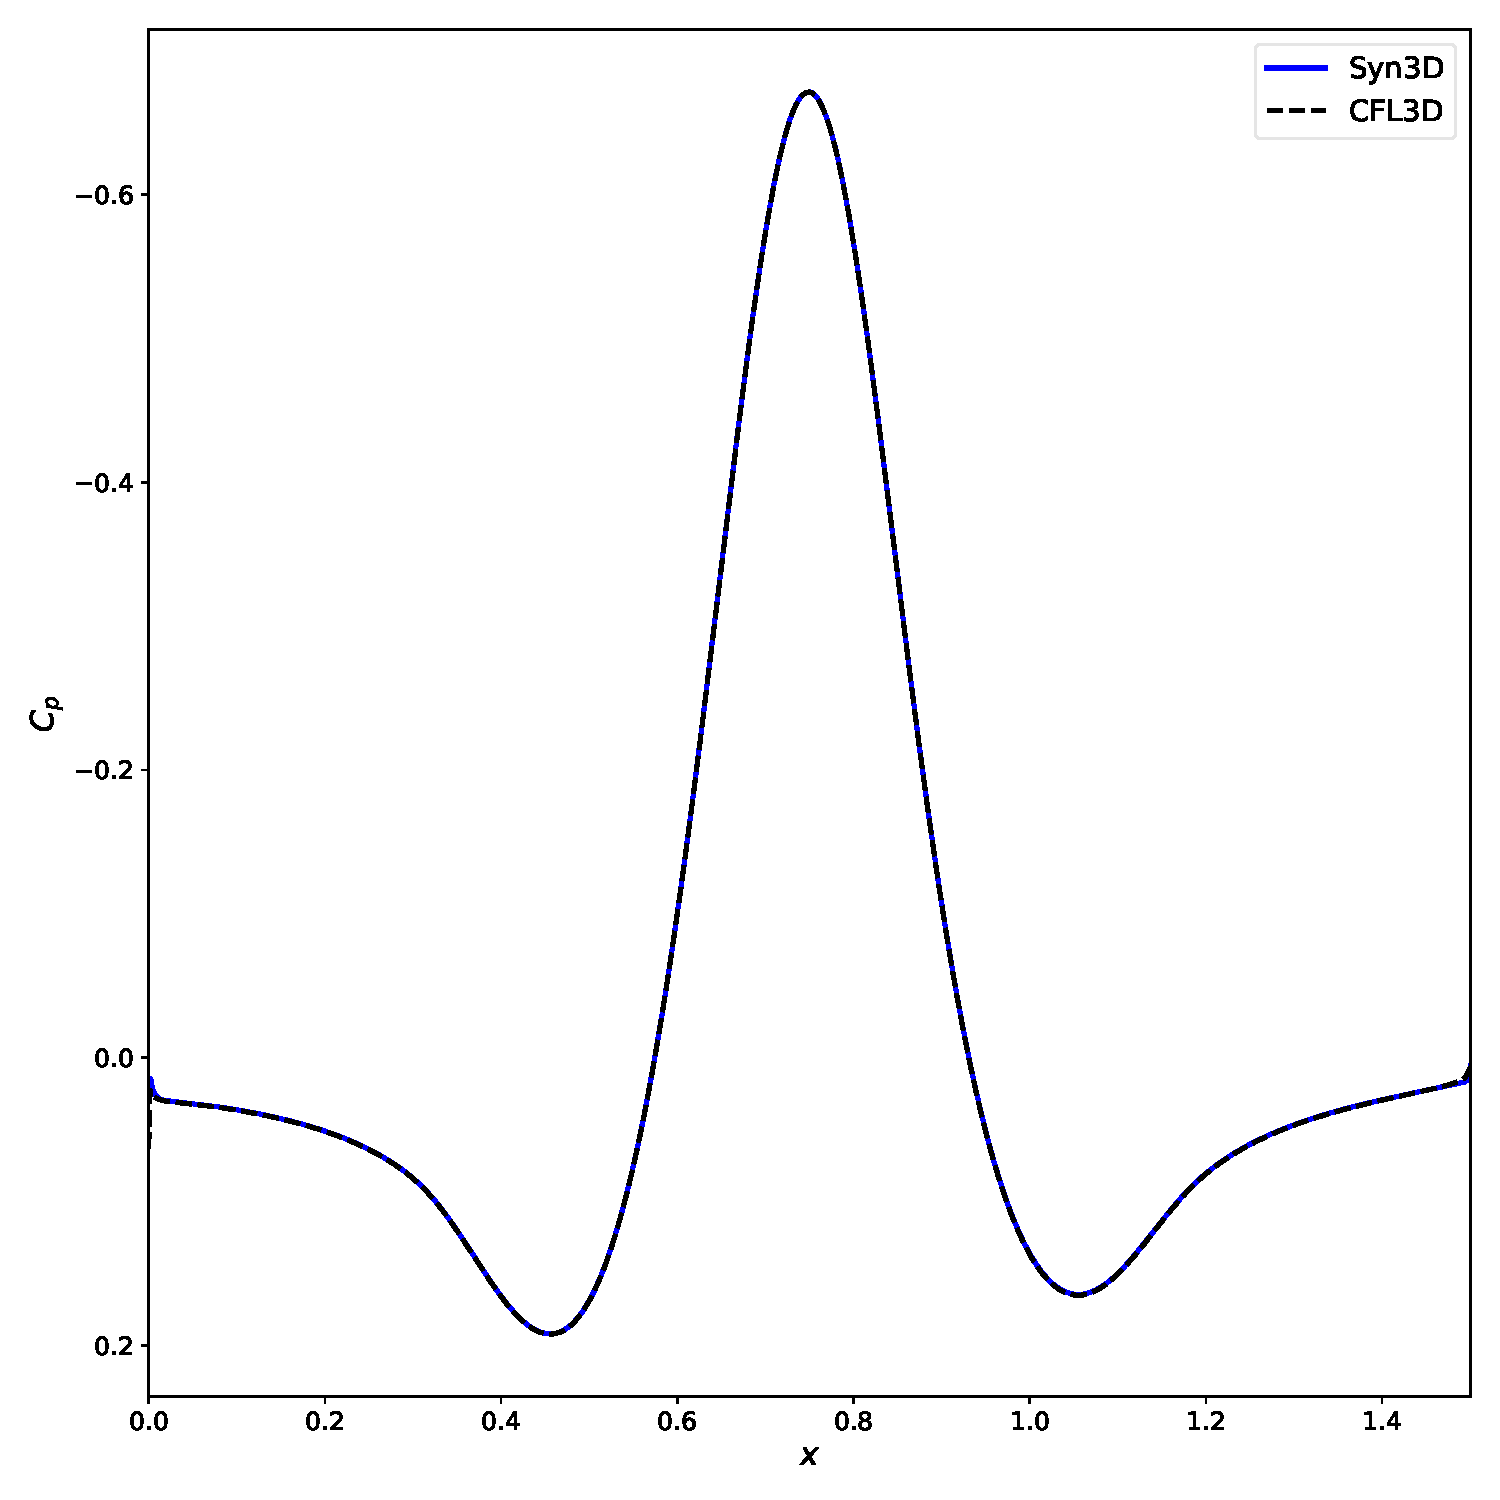
\includegraphics[width=0.7\textwidth]{figs/2dbump/CoefficientPressure.pdf}
    \caption{2D Bump (syn3D): Coefficient of pressure distribution along the bump.}
    \label{fig:syn2dbumpcp}
\end{figure}


\begin{figure}[ht!]
\centering
\begin{subfigure}{.45\textwidth}
  \centering
  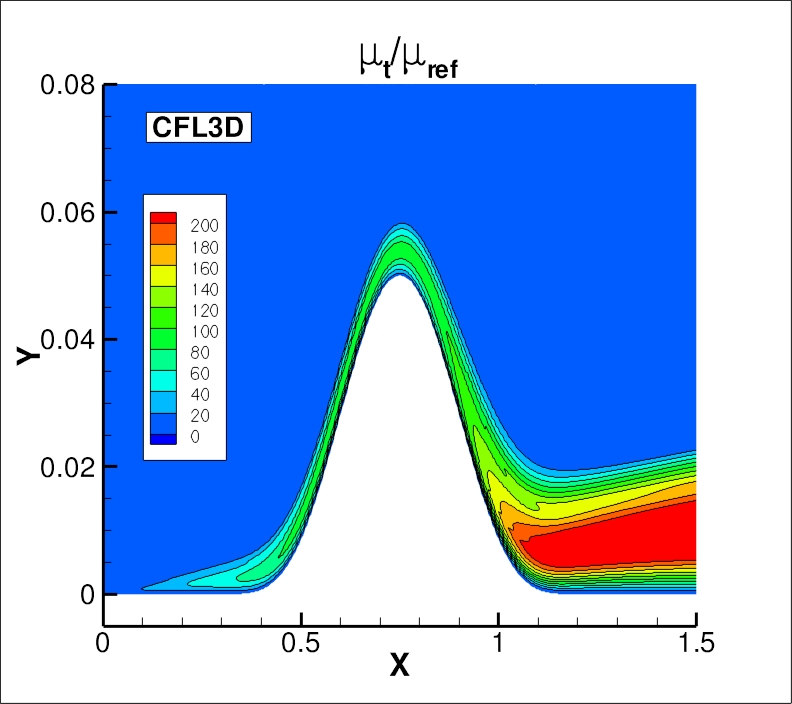
\includegraphics[width=1.0\textwidth]{figs/2dbump/MutNASA.jpg}
  \caption{CFL3D}
\end{subfigure}%
\begin{subfigure}{.45\textwidth}
  \centering
  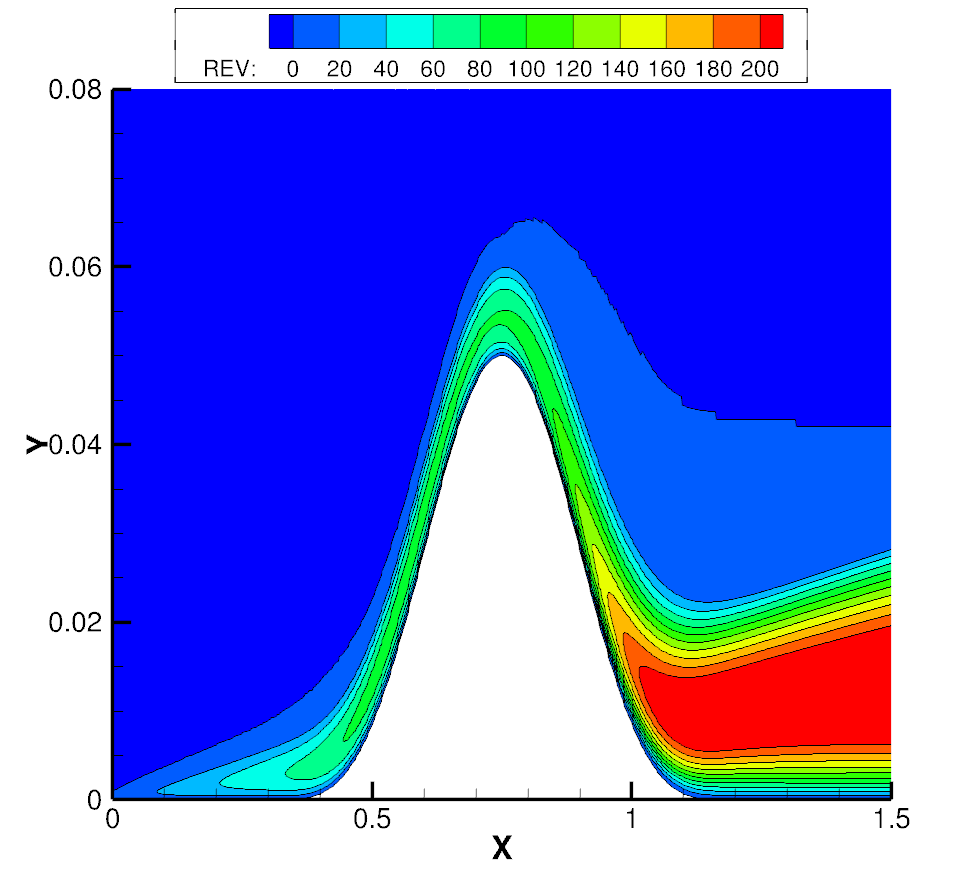
\includegraphics[width=1.0\textwidth]{figs/2dbump/RevContour2.png}
  \caption{syn3D}
\end{subfigure}
\caption{2D Bump (syn3D): Contours of $\mu_T/\mu_{\infty}$.}
\label{fig:syn2dbumpmutcontour}
\end{figure}

\begin{figure}[ht!]
\centering
\begin{subfigure}{.45\textwidth}
  \centering
  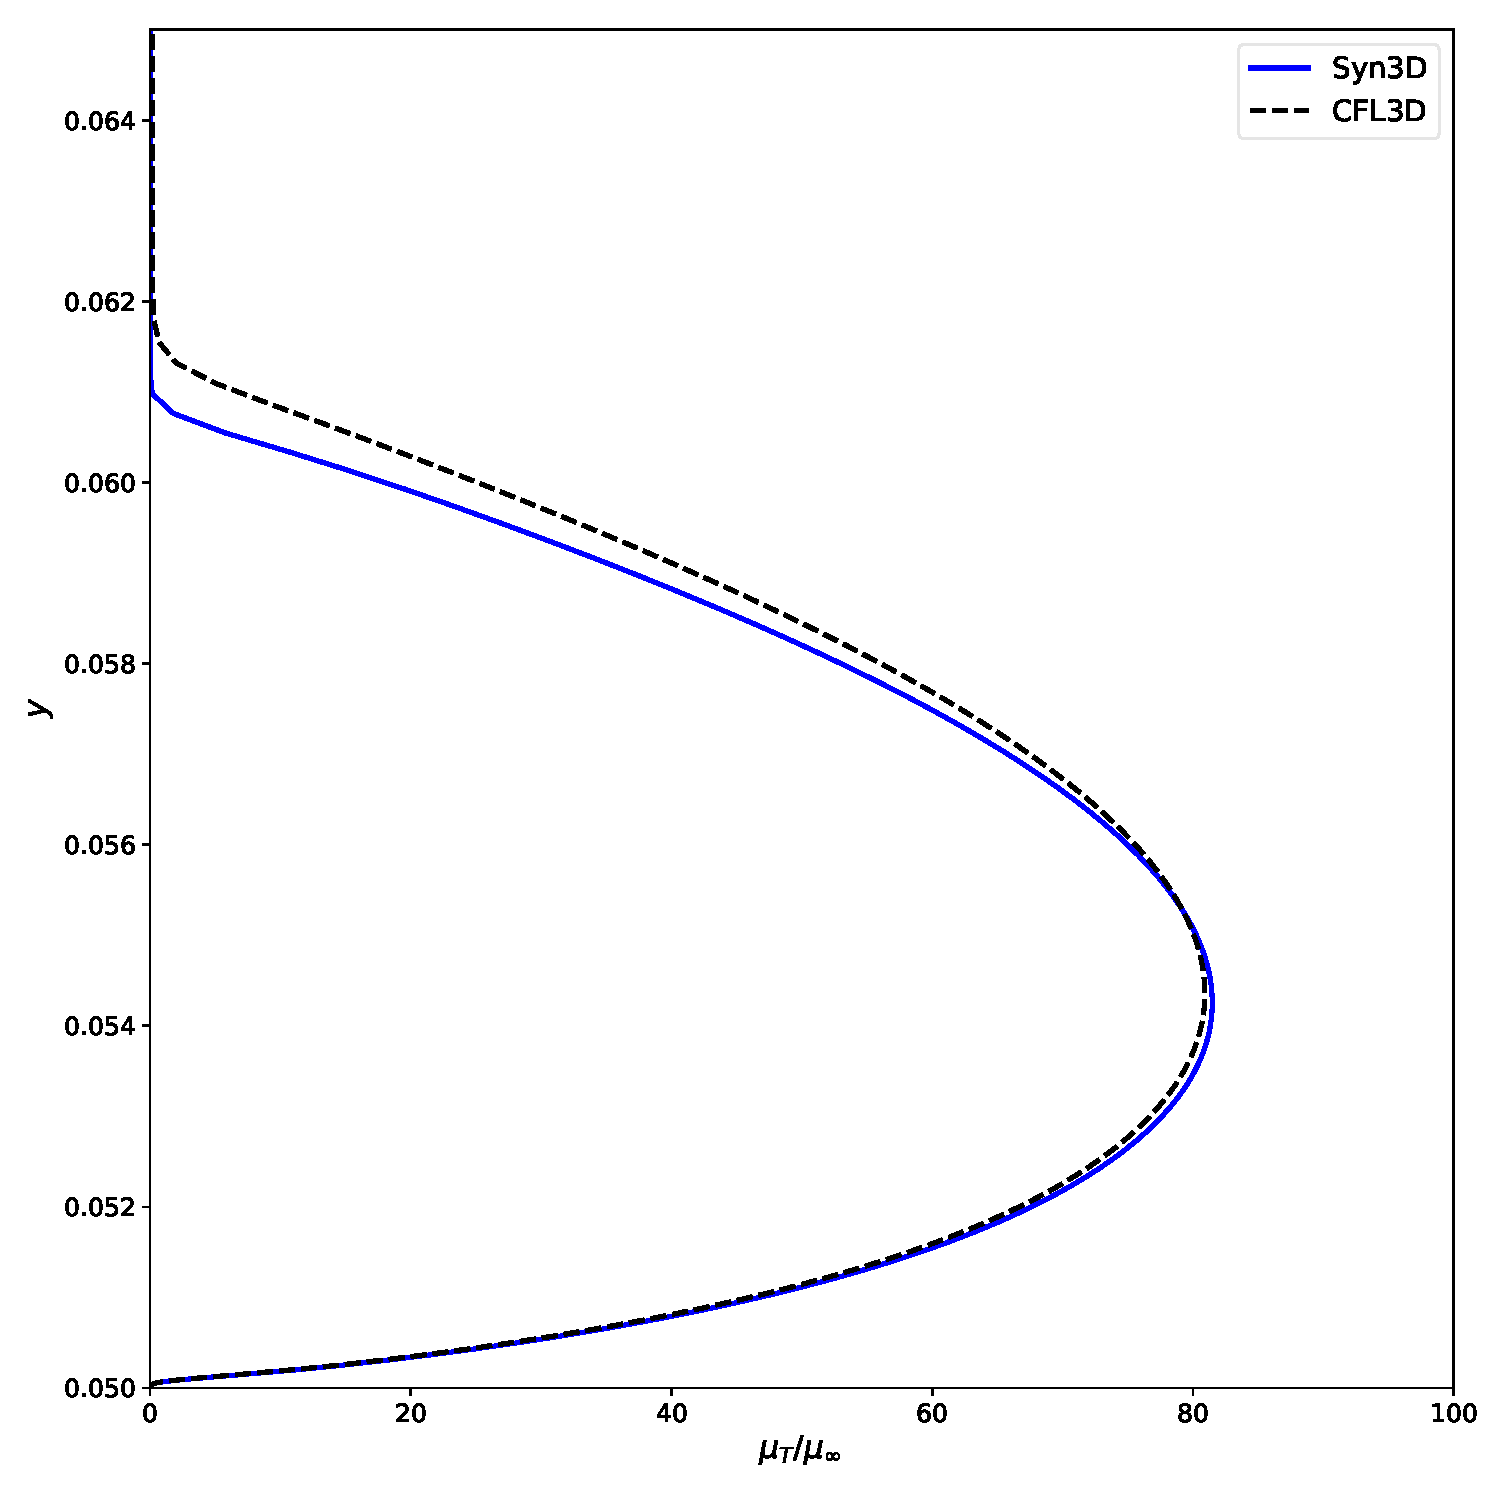
\includegraphics[width=1.0\textwidth]{figs/2dbump/revBL.pdf}
  \caption{Profile at $x=0.75$}
  \label{fig:syn2dbumpmutprof}
\end{subfigure}%
\begin{subfigure}{.45\textwidth}
  \centering
  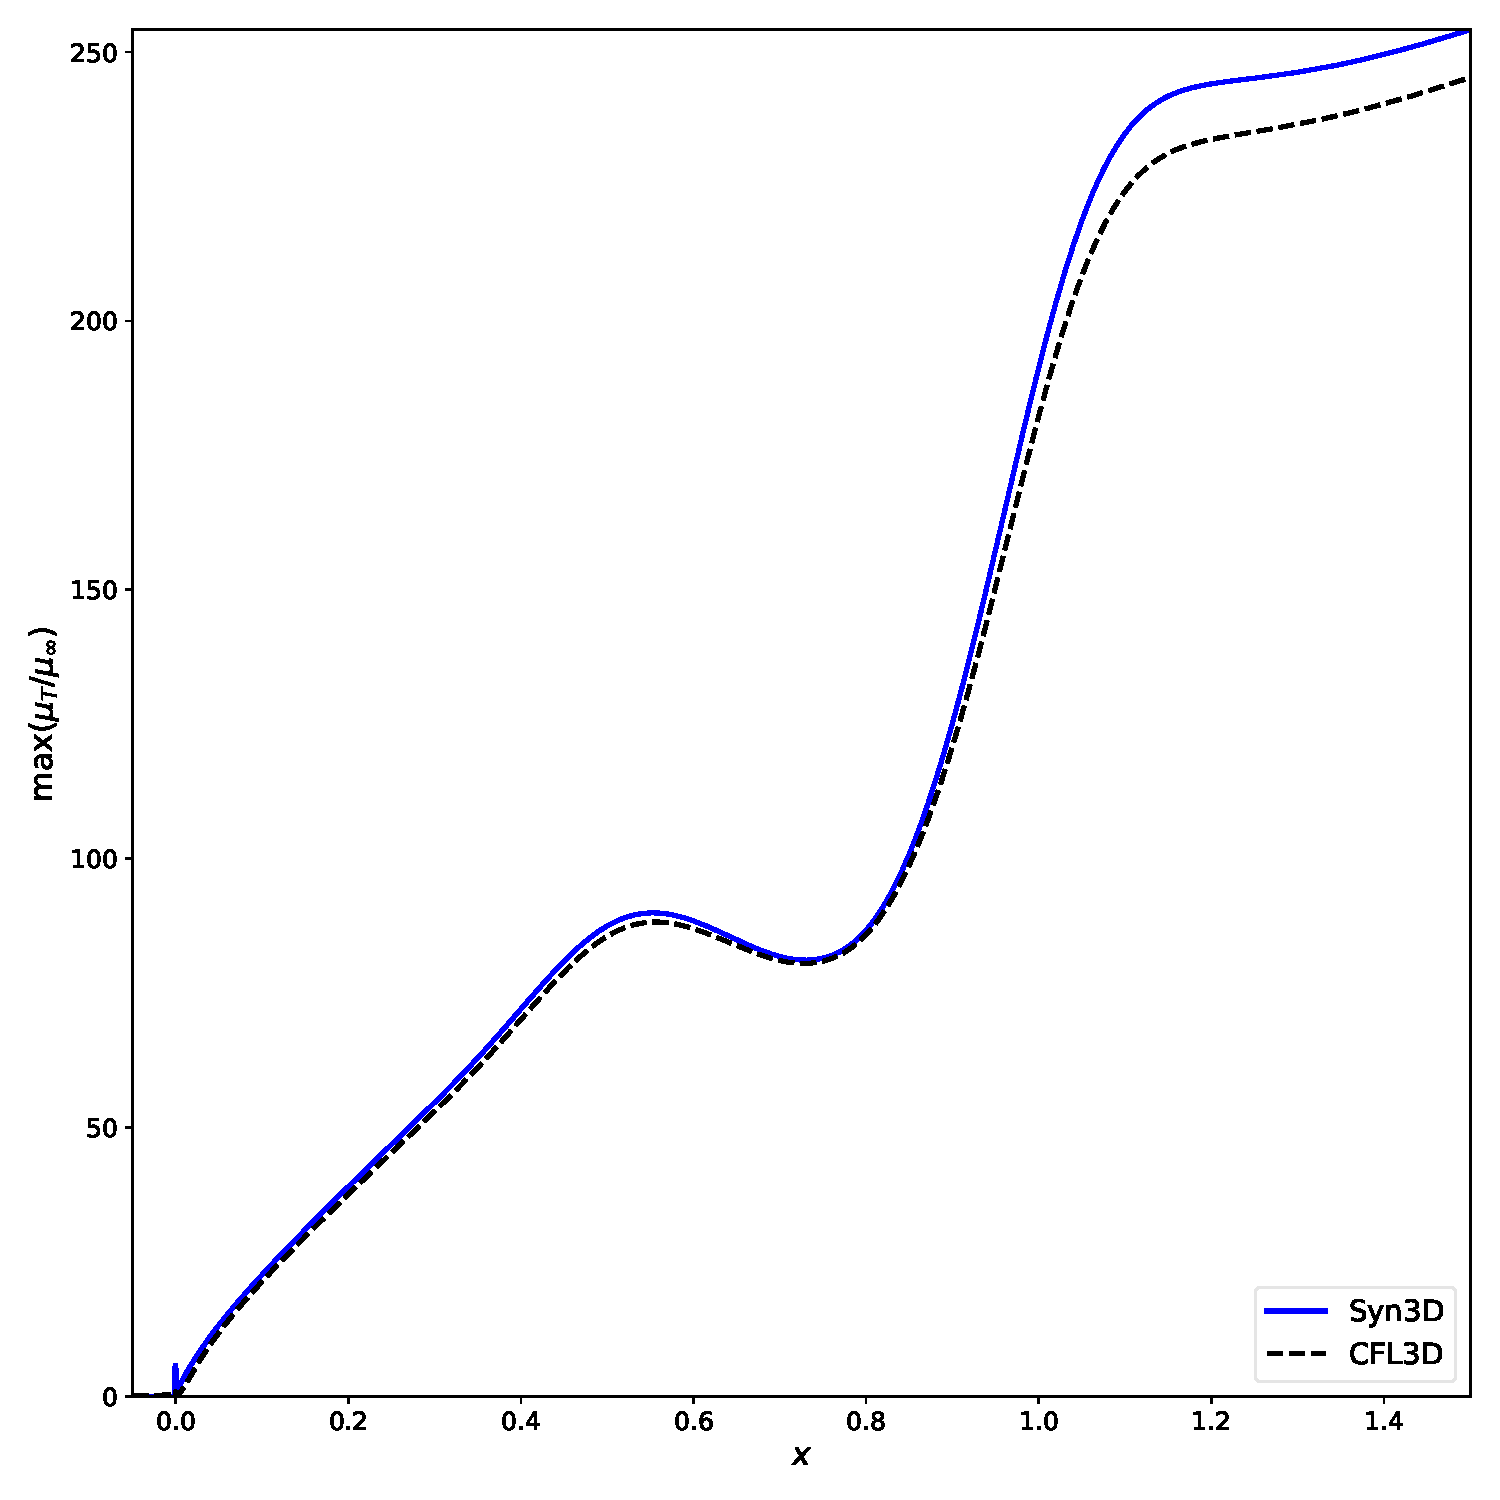
\includegraphics[width=1.0\textwidth]{figs/2dbump/maxRev.pdf}
  \caption{Maximum value in the boundary layer.}
  \label{fig:syn2dbumpmaxmut}
\end{subfigure}
\caption{2D Bump (syn3D): Dimensionless eddy viscosity profiles.}
\label{fig:syn2dbumpmut}
\end{figure}

\begin{figure}[ht!]
\centering
\begin{subfigure}{.45\textwidth}
  \centering
  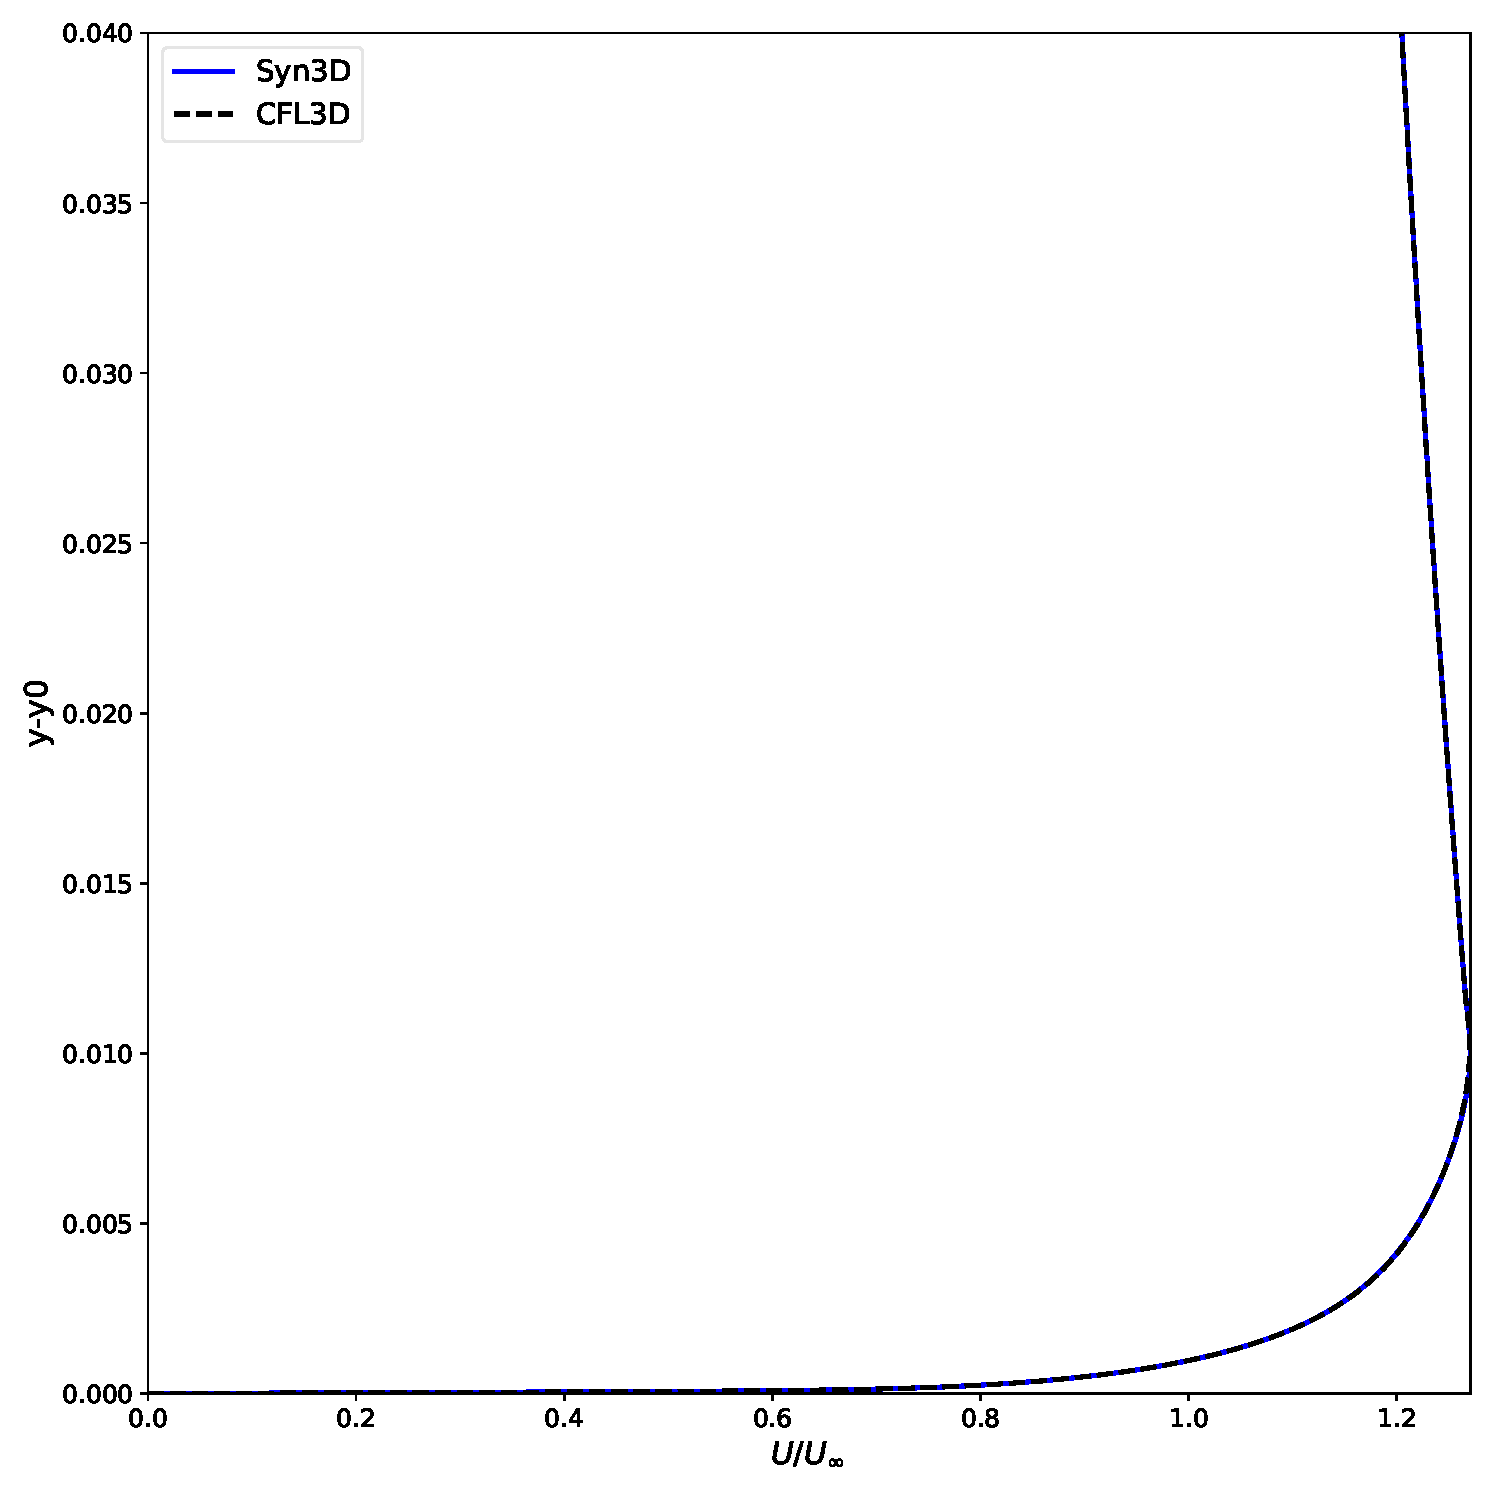
\includegraphics[width=1.0\textwidth]{figs/2dbump/u75.pdf}
  \caption{$x=0.75$}
\end{subfigure}%
\begin{subfigure}{.45\textwidth}
  \centering
  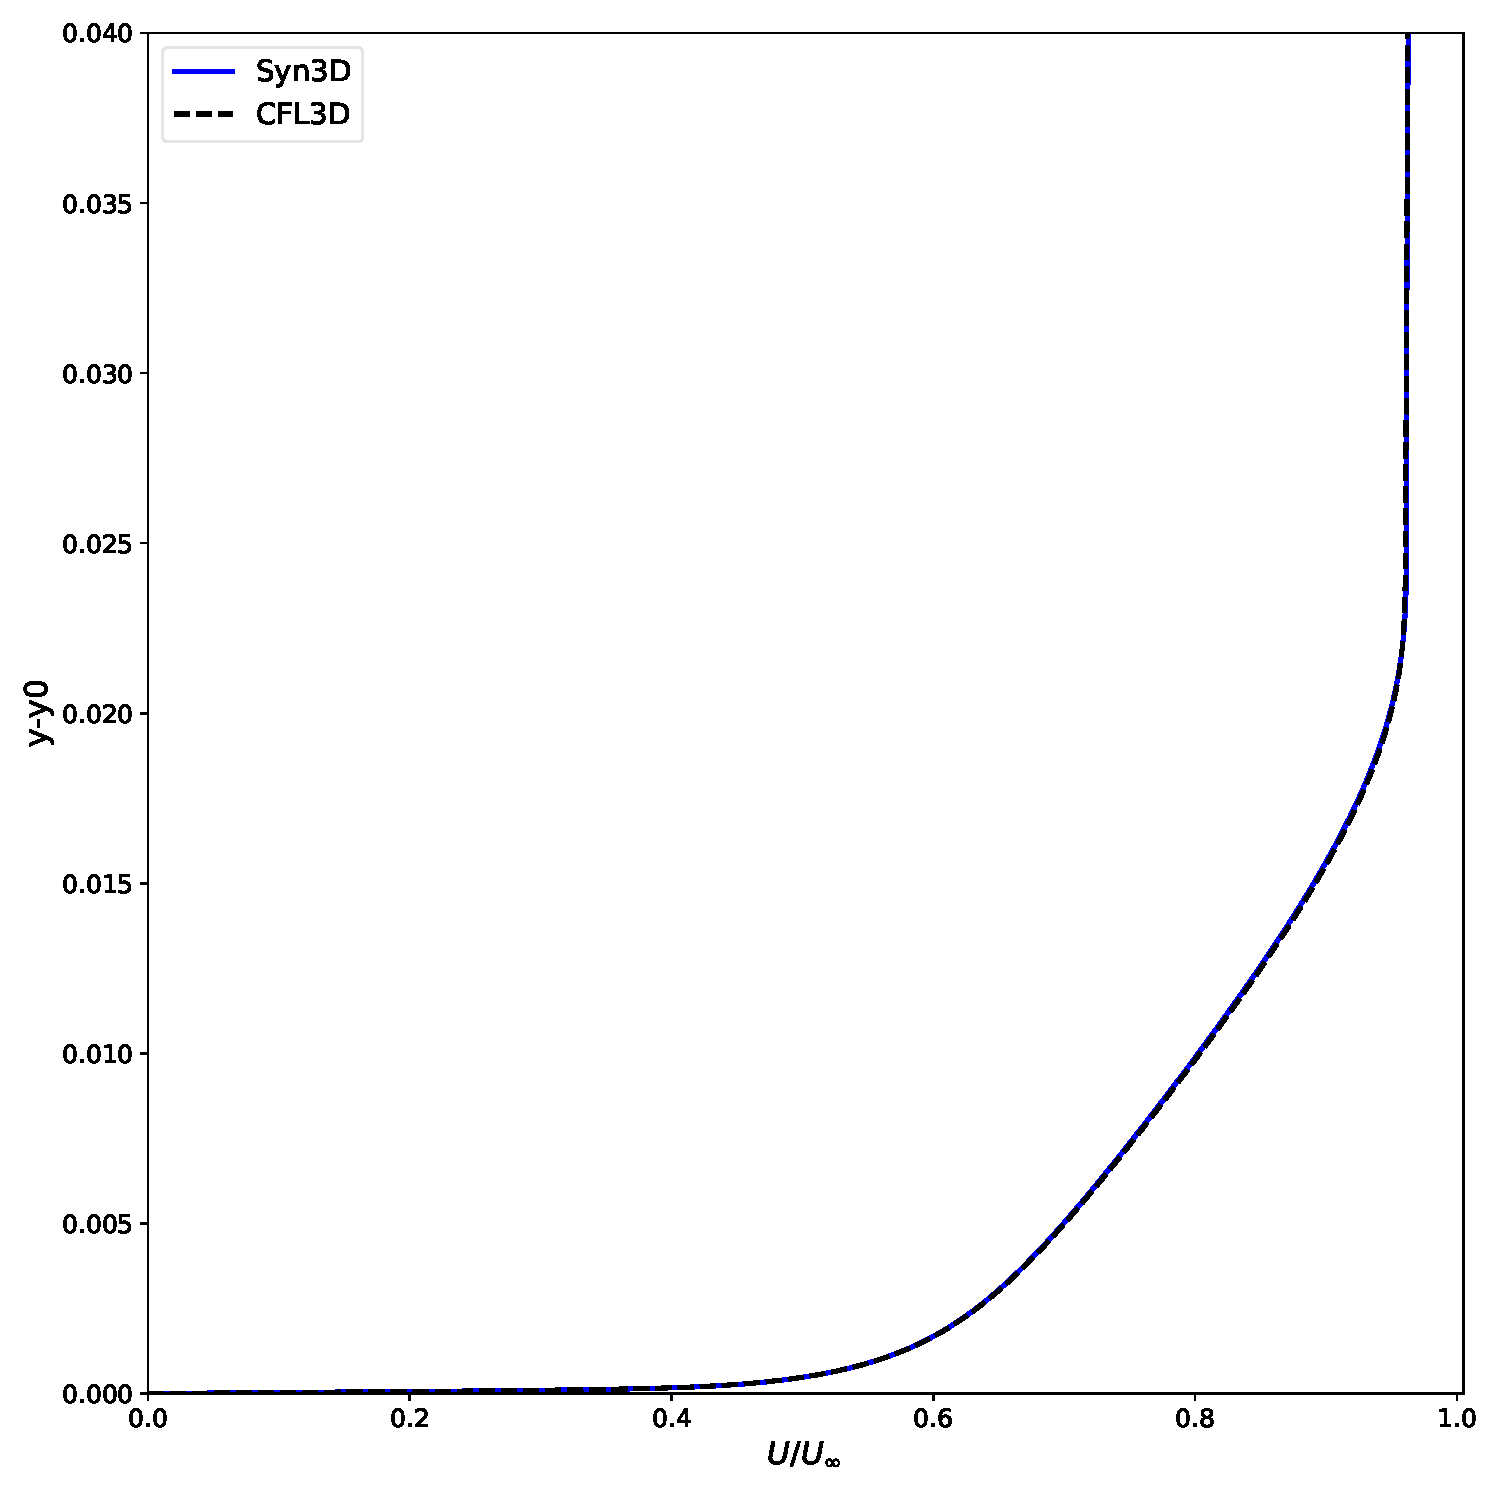
\includegraphics[width=1.0\textwidth]{figs/2dbump/u120148.pdf}
  \caption{$x=1.20148$}
\end{subfigure}
\caption{2D Bump (syn3D): Dimensionless velocity profiles $U/U_\infty$.}
\label{fig:syn2dbumpu}
\end{figure}

\Cref{fig:syn2dbumpcf} compares the $C_f$ distribution over the bump for the finest grid. The skin friction coefficient can be seen to start high, slowly decrease in the flat portion as it did for the flat plate, and then increase on the bump as it accelerates. The value of $C_f$ is under-predicted syn3D until the peak of the bump, after which point it is over-predicted.

\Cref{fig:syn2dbumpcp} shows the $C_p$ distribution. The trend in this plot is similar to the skin friction plot. The pressure decreases as the flow accelerates at the leading edge of the bump. The pressure then increases again once the peak is reached. The pressure coefficient is identical between syn3D and CFL3D, as is the drag force due to the pressure component $C_{Dp}$ (see~\Cref{tab:syn2dbump1}).

\Cref{fig:syn2dbumpmutcontour} compares the contour of eddy viscosity over the bump. Both contour plots show similar trends. However, values of $\mu_t$ in the downstream region are slightly elevated for syn3D.

\Cref{fig:syn2dbumpmut} compares the eddy viscosity through line plots. Similar to the flat plate, $\mu_t$ increases with $x$. Once again, syn3D displays a small peak in eddy viscosity at the leading edge ($x=0.0$). The difference of the maximum $\mu_t$ value between syn3D and CFL3D is, as mentioned previously, greater in the downstream region. In, \Cref{fig:syn2dbumpmutprof}, it can again be seen that the eddy viscosity increases with $y$ until it reaches a maximum value and begins to decrease again as it reaches the far-field region. In the region of increasing $\mu_t$ ($y < 0.054$), syn3D and CFL3D show very similar results. In the decreasing region, however, syn3D displays a greater gradient and under-predicts the distance needed for $\mu_t$ to return to its free-stream value.

\Cref{fig:syn2dbumpu} compares the velocity profile. A sharp velocity gradient near the wall is observed at both locations, although the height of the boundary layer is greater as $x$ increases. Profiles are identical between the two solvers.
\begin{figure}[ht!]
\centering
  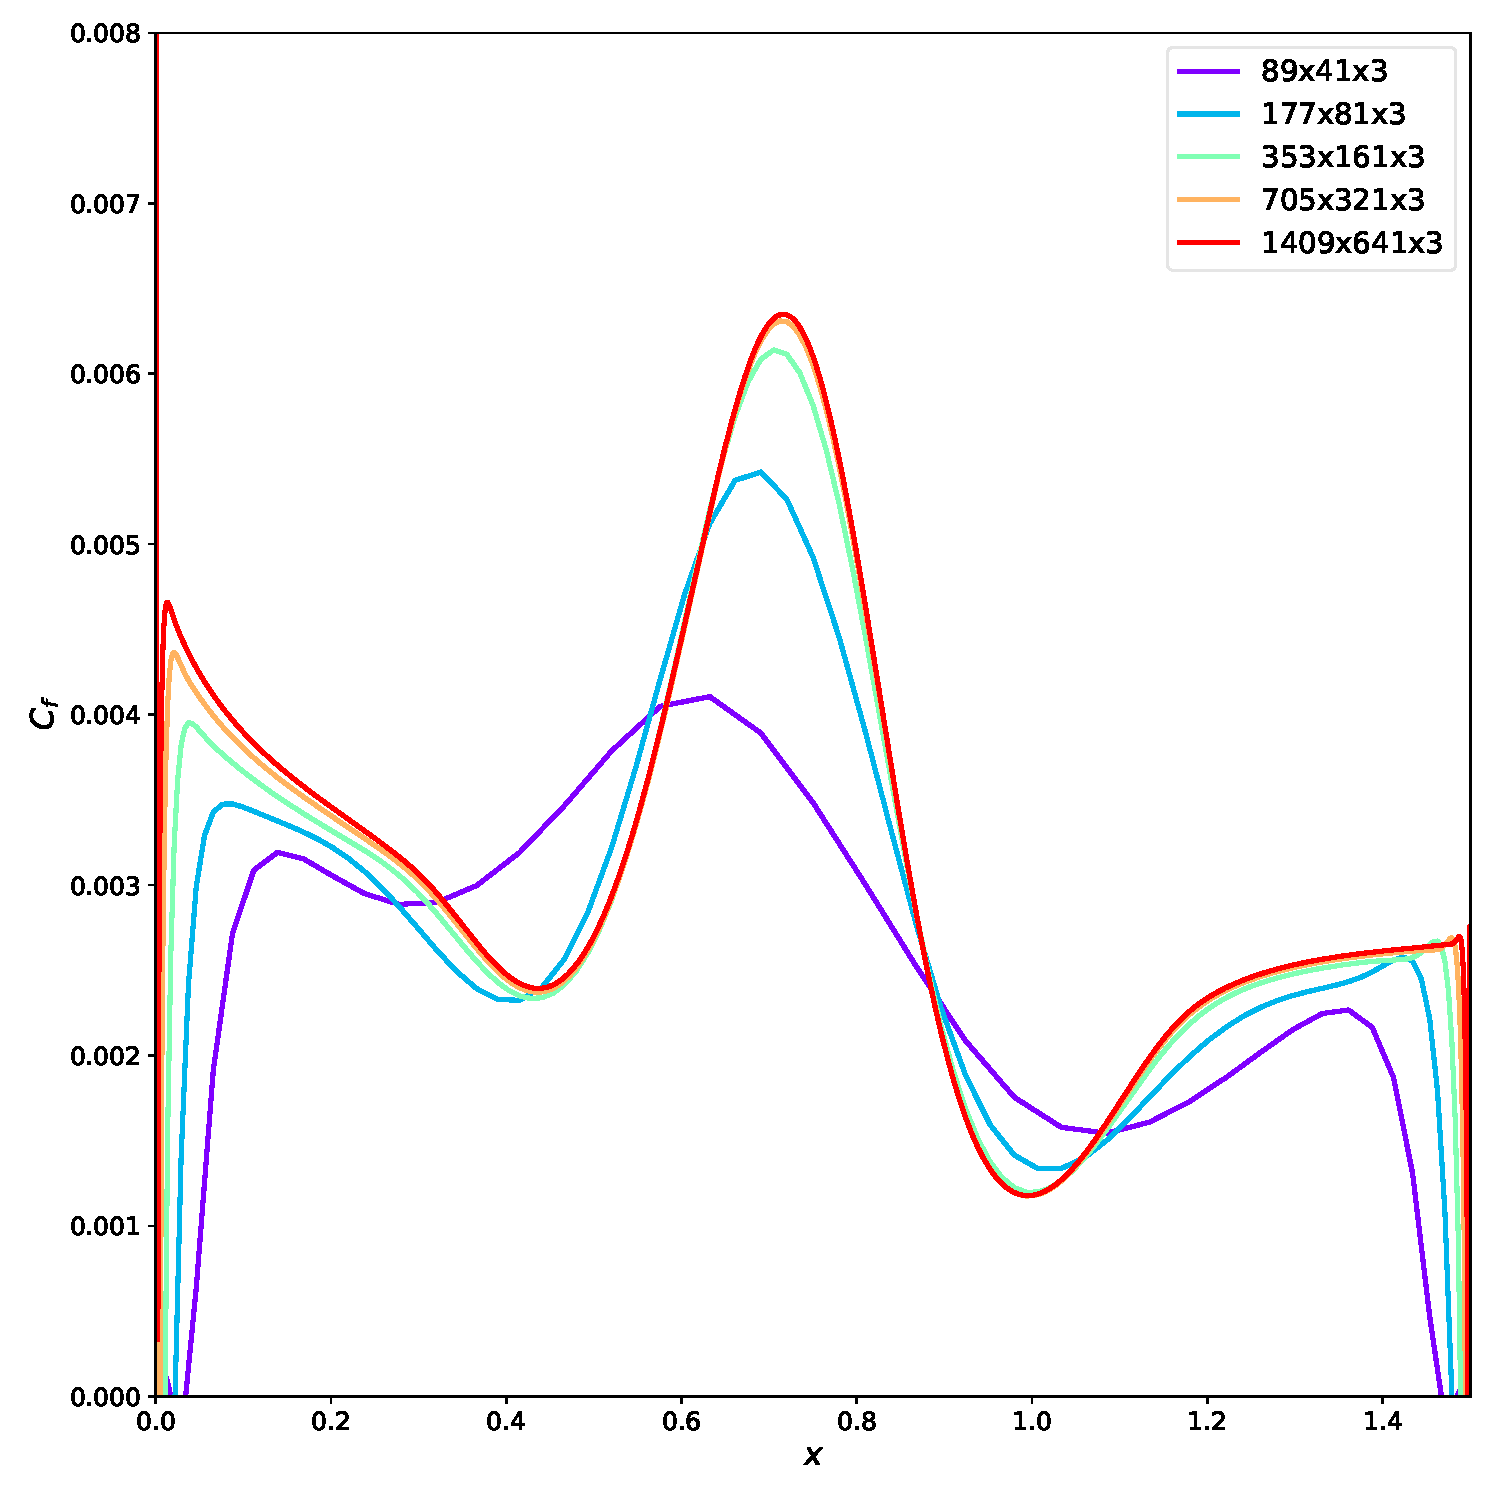
\includegraphics[width=0.7\textwidth]{figs/2dbump/CfGridStudy.pdf}
    \caption{2D Bump (syn3D): Coefficient of skin friction along the bump for various grids.}
    \label{fig:syn2dbumpcfstudy}
\end{figure}

\begin{figure}[ht!]
\centering
  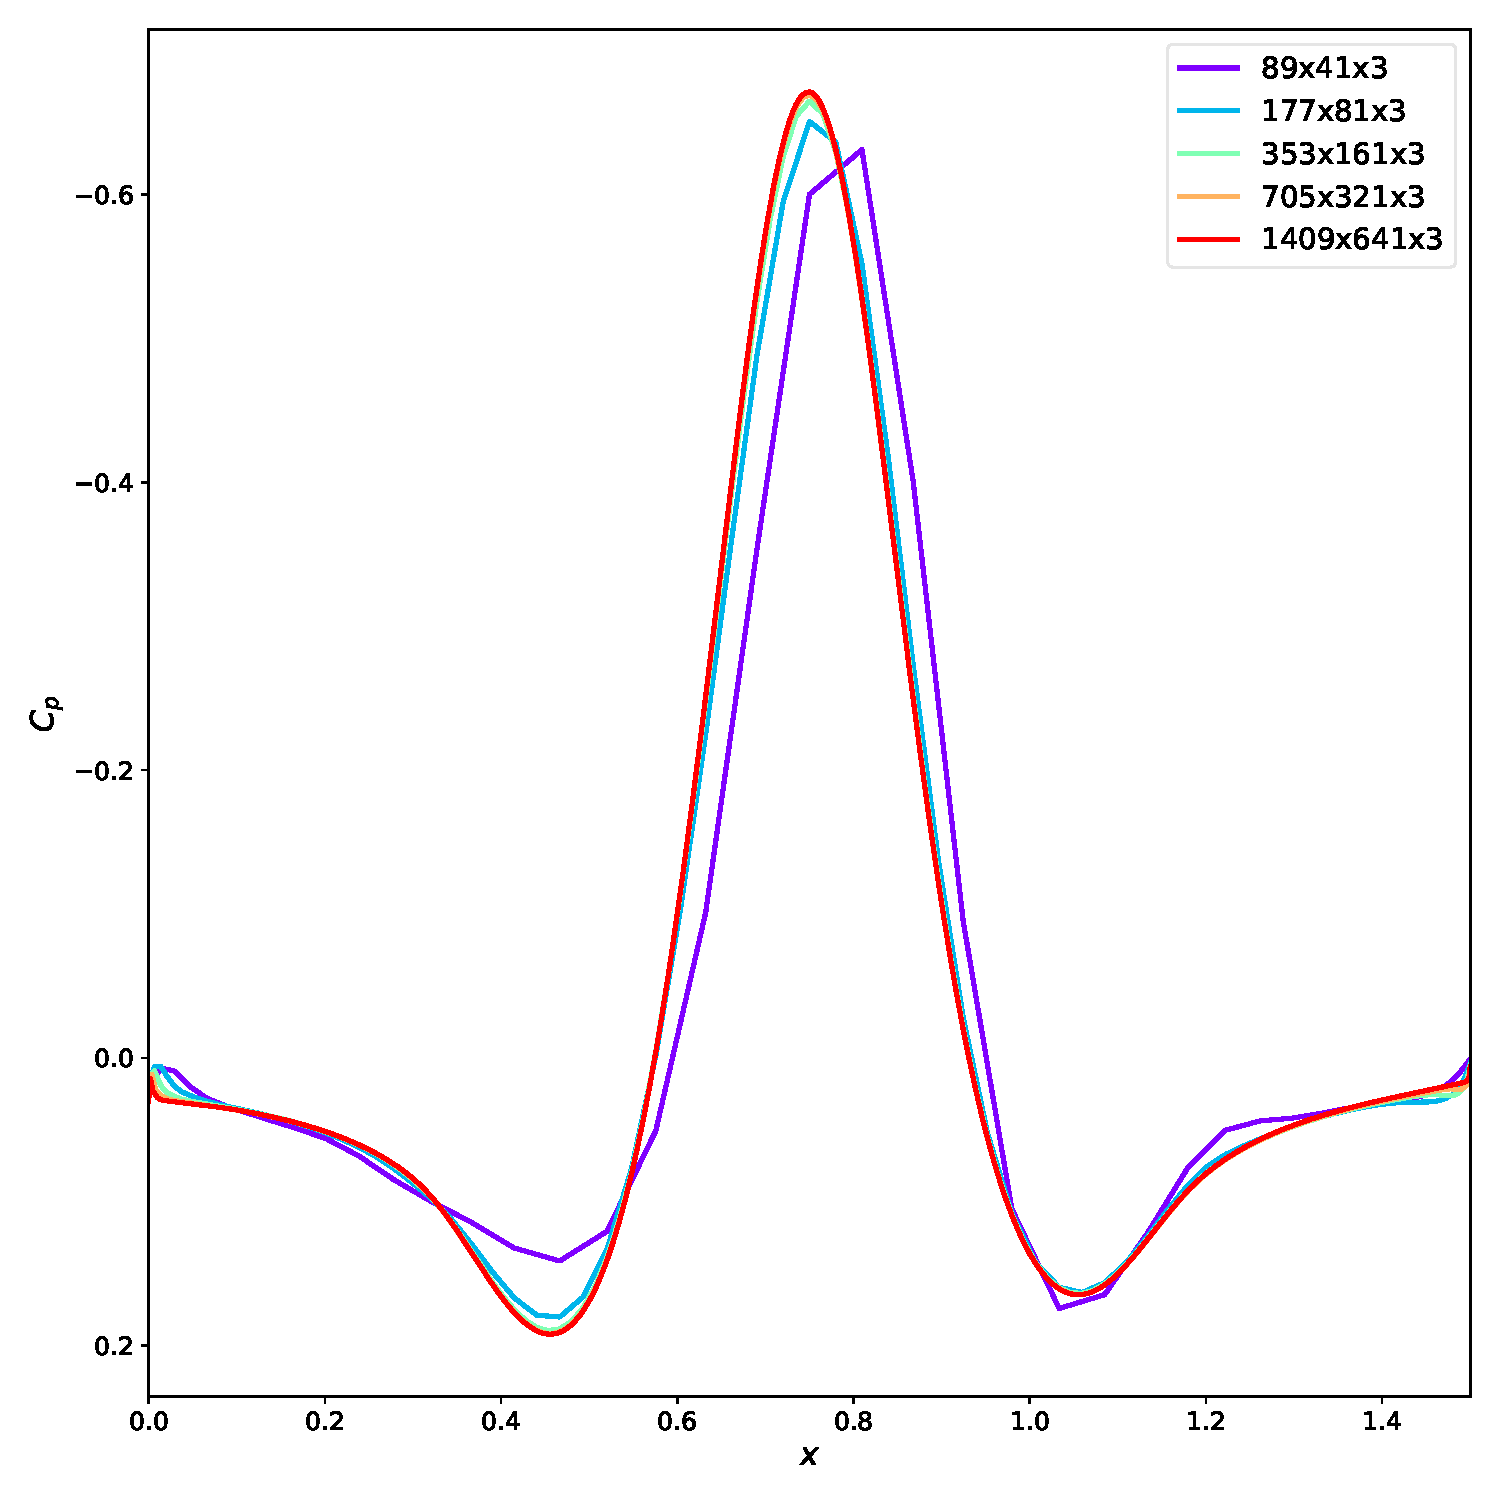
\includegraphics[width=0.7\textwidth]{figs/2dbump/CpGridStudy.pdf}
    \caption{2D Bump (syn3D): Coefficient of pressure along the bump for various grid.}
    \label{fig:syn2dbumpcpstudy}
\end{figure}

\begin{figure}[ht!]
\centering
\begin{subfigure}{.45\textwidth}
  \centering
  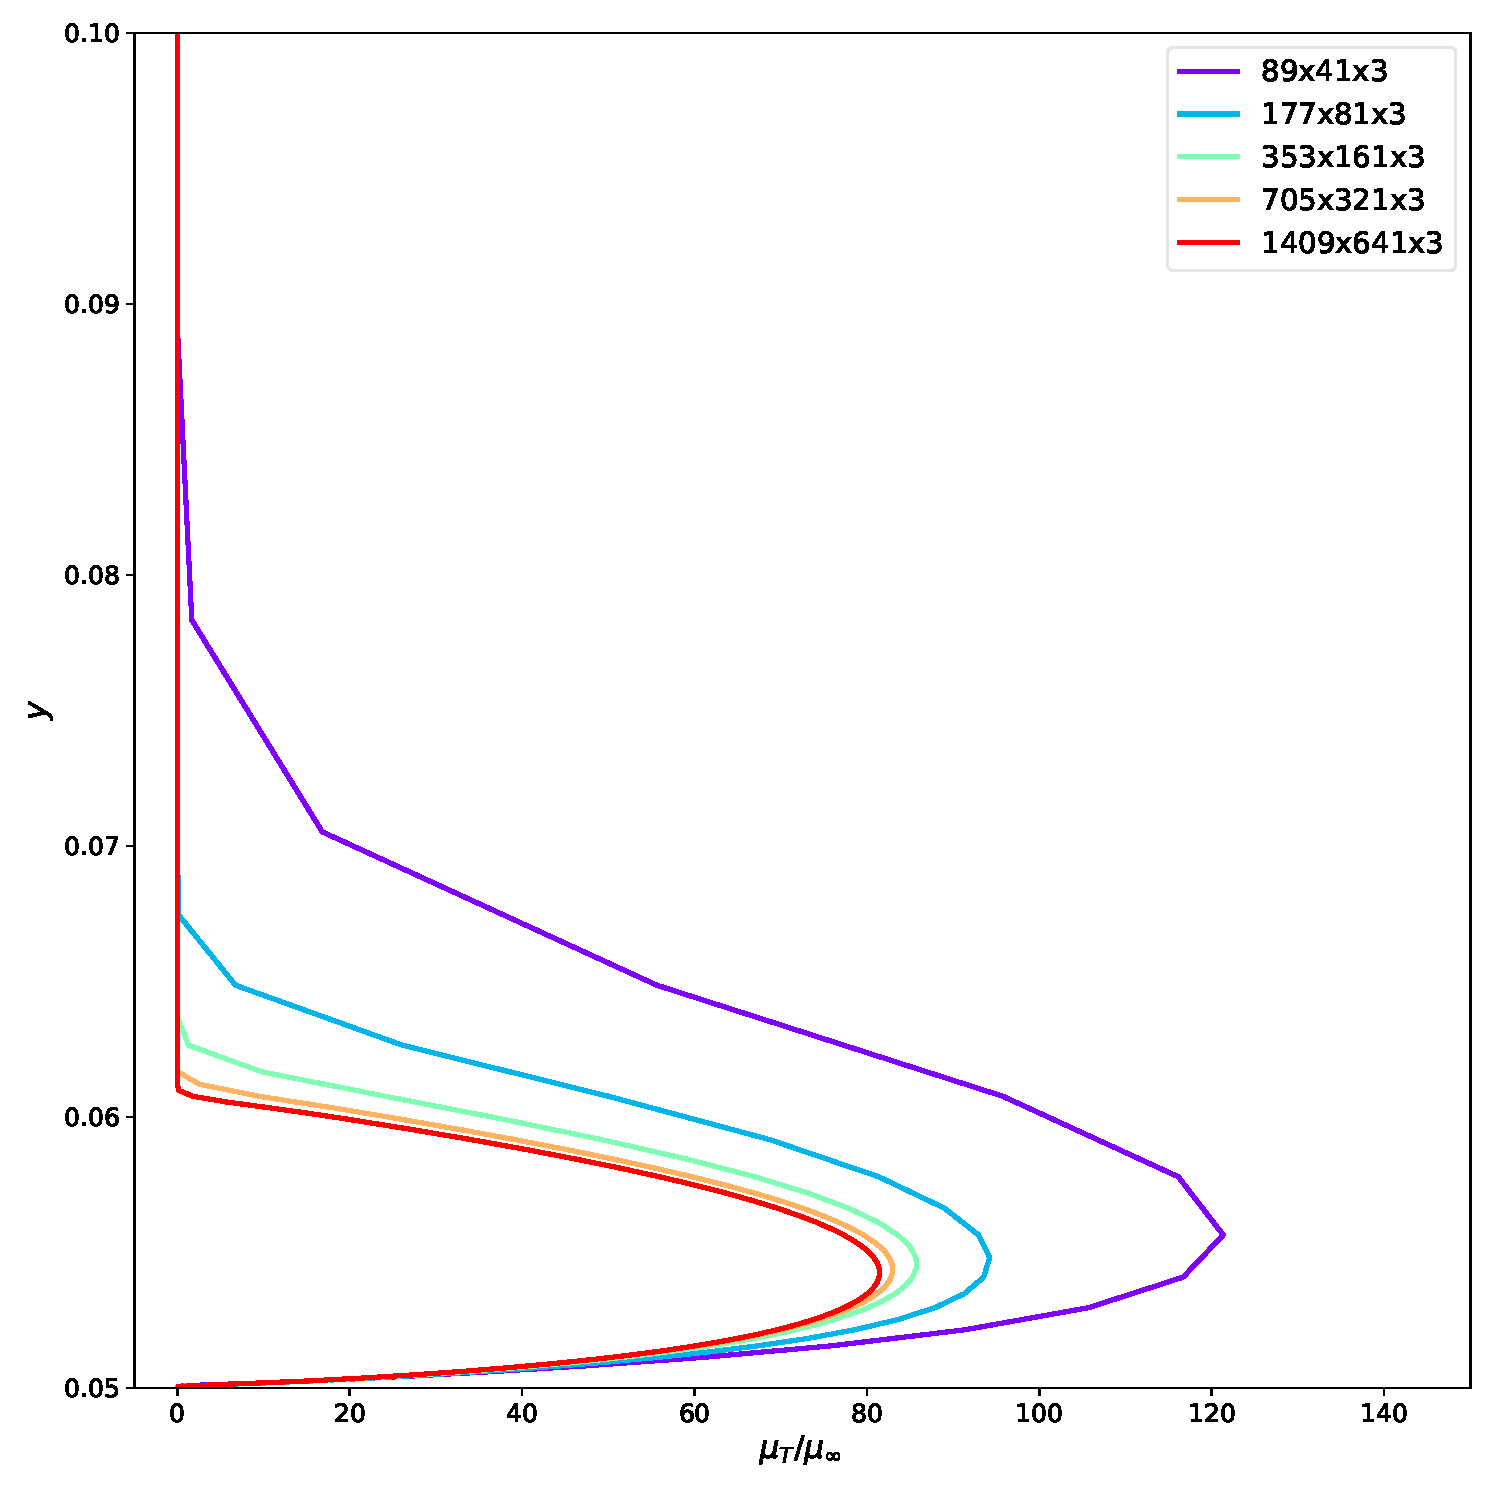
\includegraphics[width=1.0\textwidth]{figs/2dbump/revBLGridStudy.pdf}
  \caption{Profile at $x=0.75$.}
\end{subfigure}%
\begin{subfigure}{.45\textwidth}
  \centering
  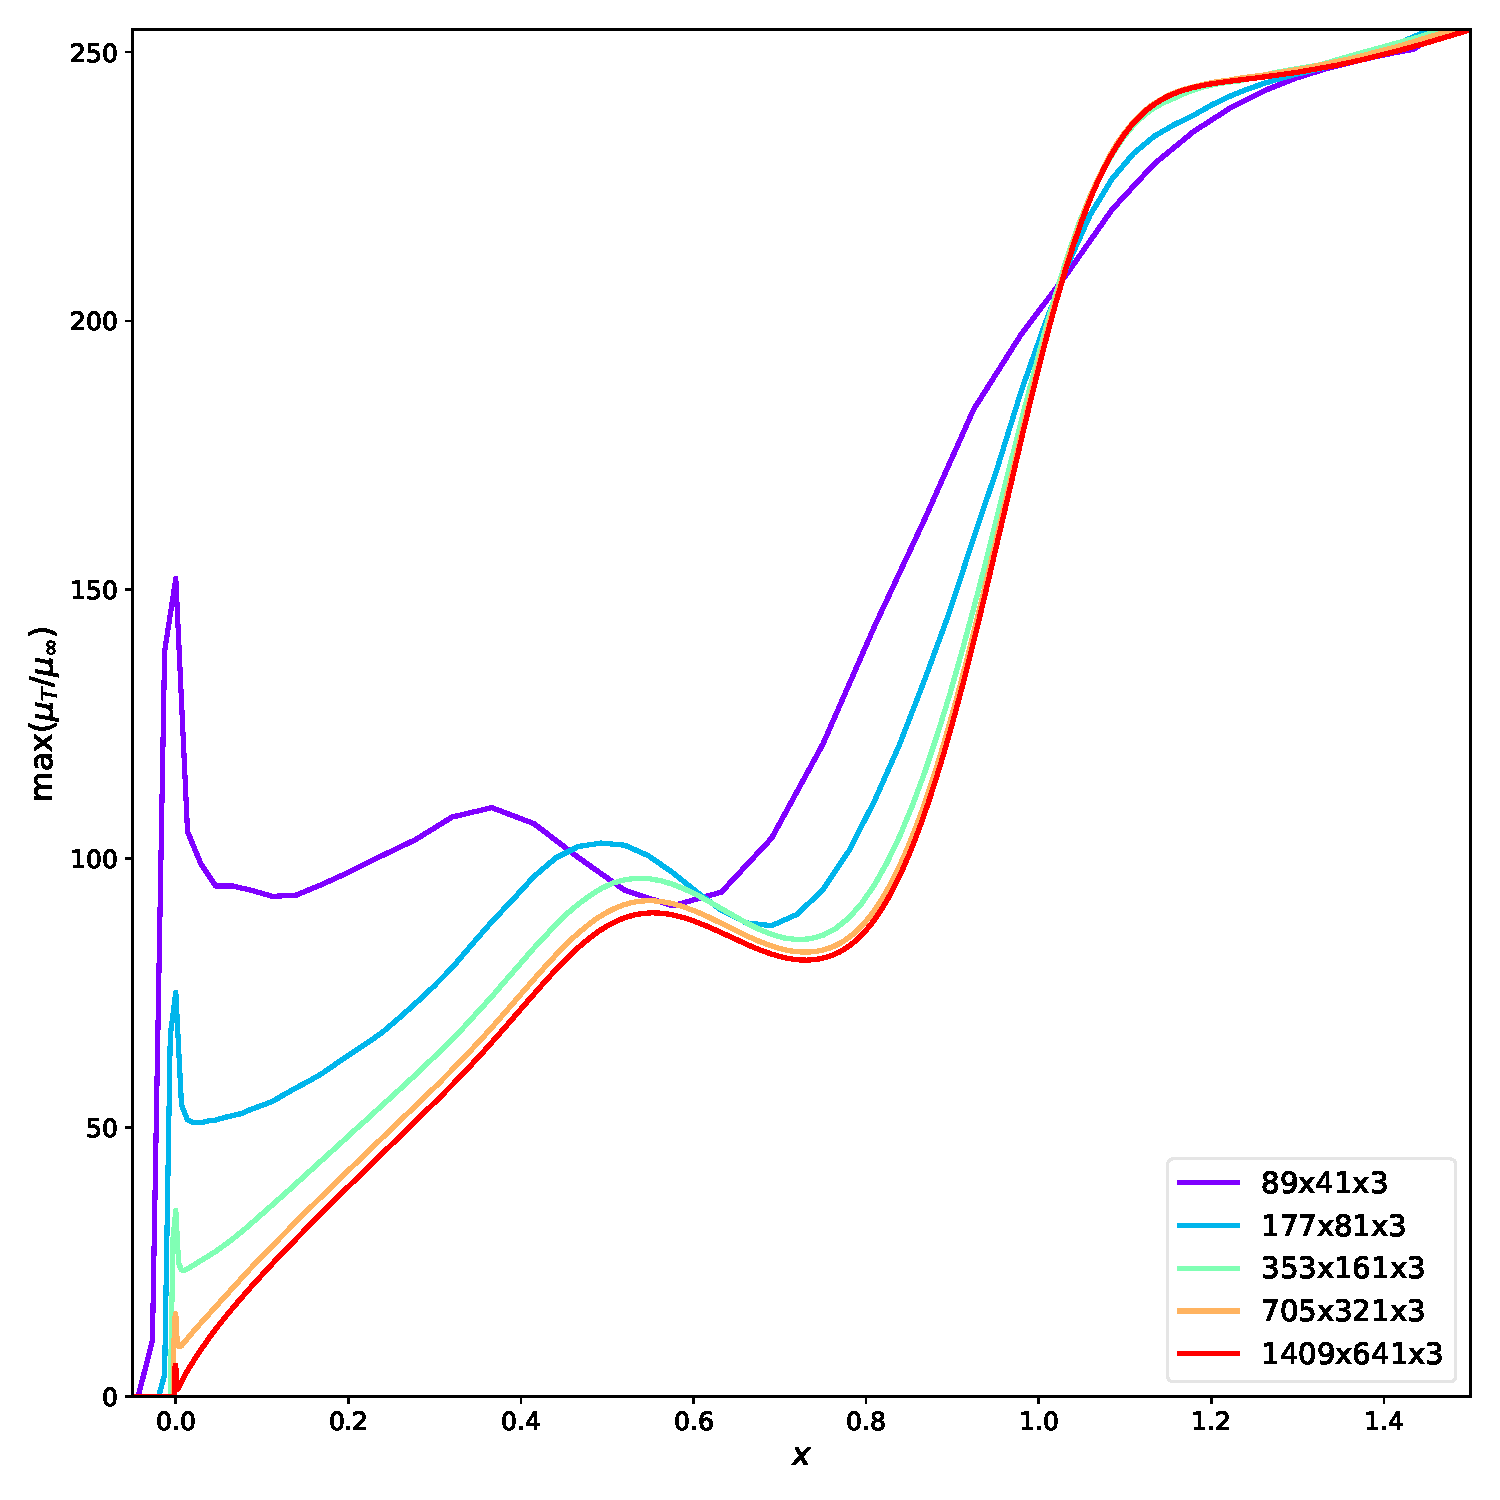
\includegraphics[width=1.0\textwidth]{figs/2dbump/maxRevstudy.pdf}
  \caption{Maximum value in the boundary layer.}
\end{subfigure}
\caption{2D Bump (syn3D): Dimensionless eddy viscosity profiles on the bump for various grids.}
\label{fig:syn2dbumpmutstudy}
\end{figure}

\begin{figure}[ht!]
\centering
\begin{subfigure}{.45\textwidth}
  \centering
  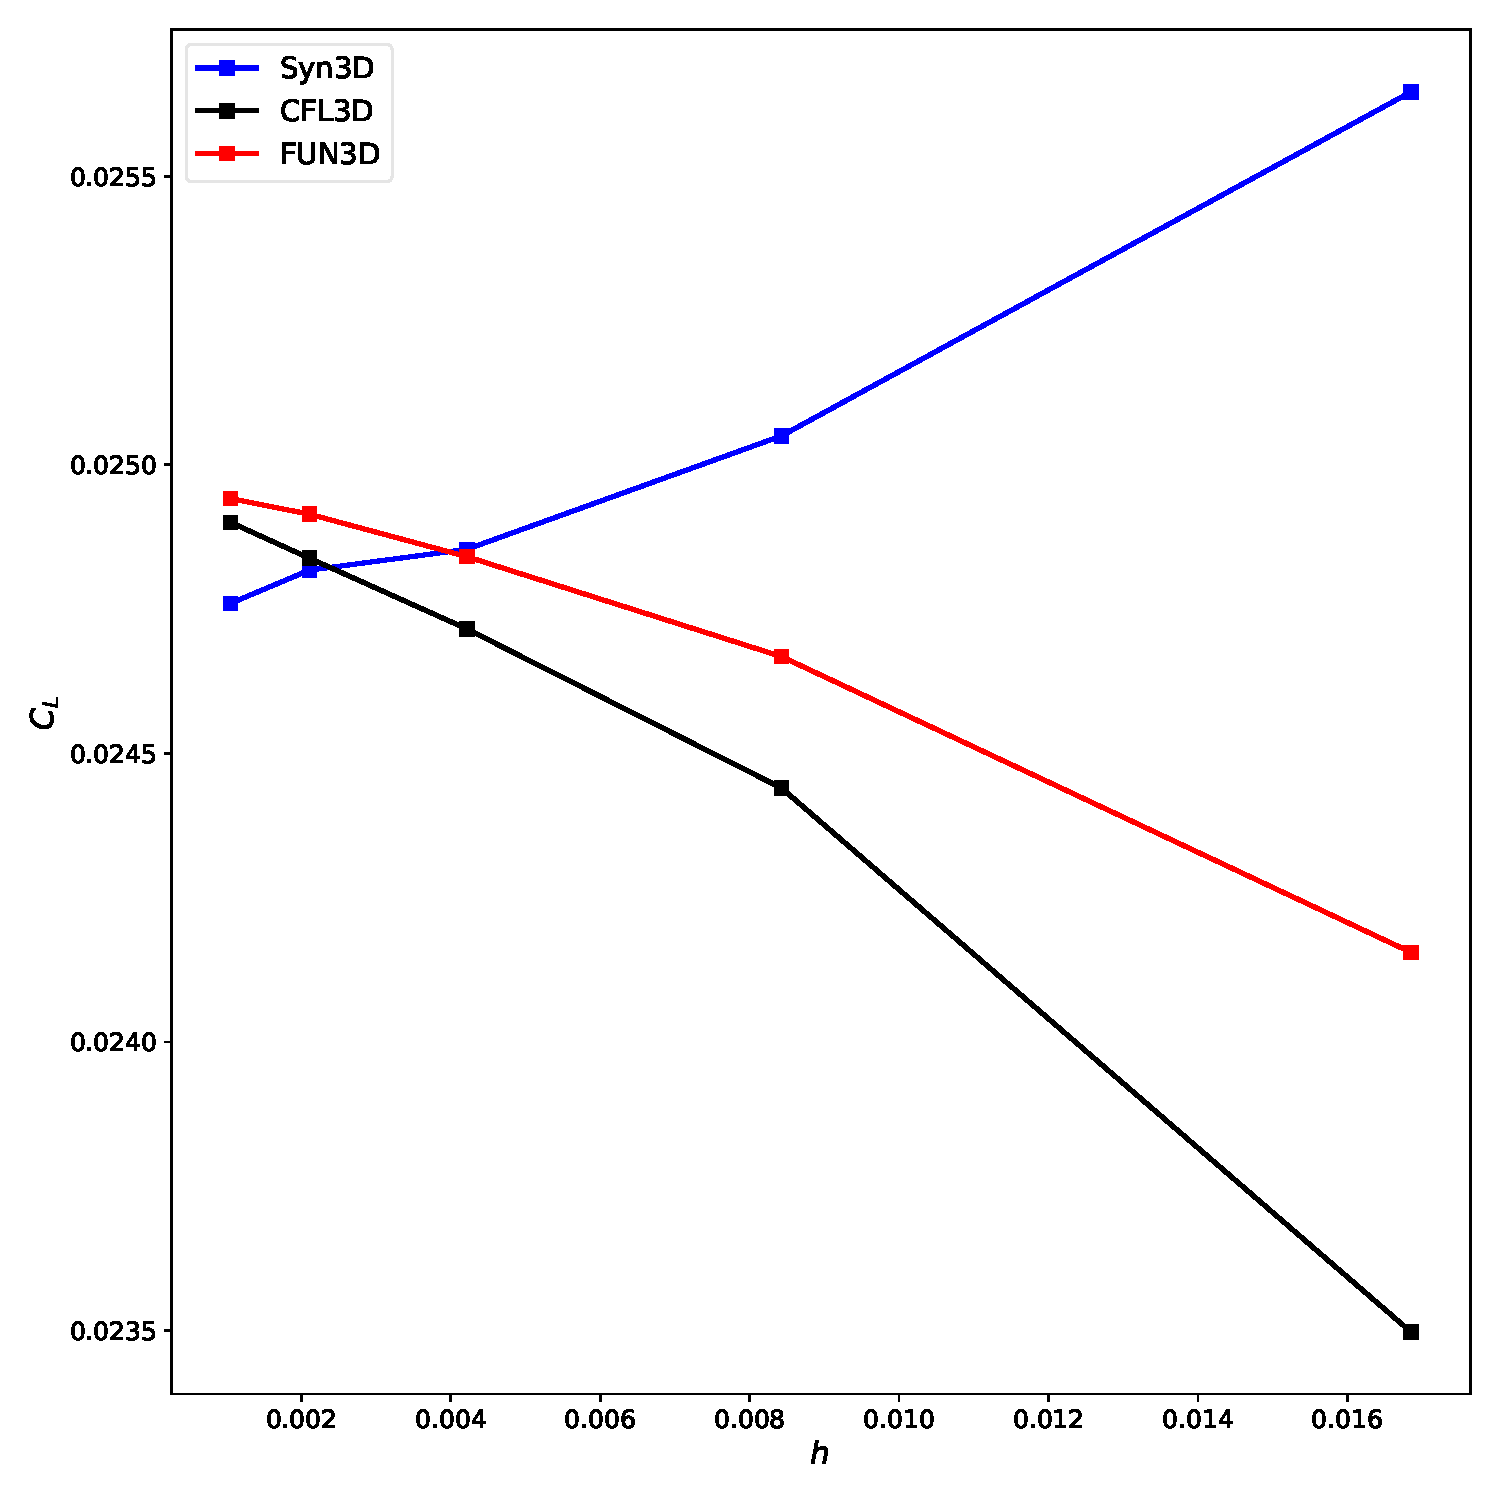
\includegraphics[width=1.0\textwidth]{figs/2dbump/C_LGridStudy.pdf}
  \caption{Lift coefficient.}
\end{subfigure}%
\begin{subfigure}{.45\textwidth}
  \centering
  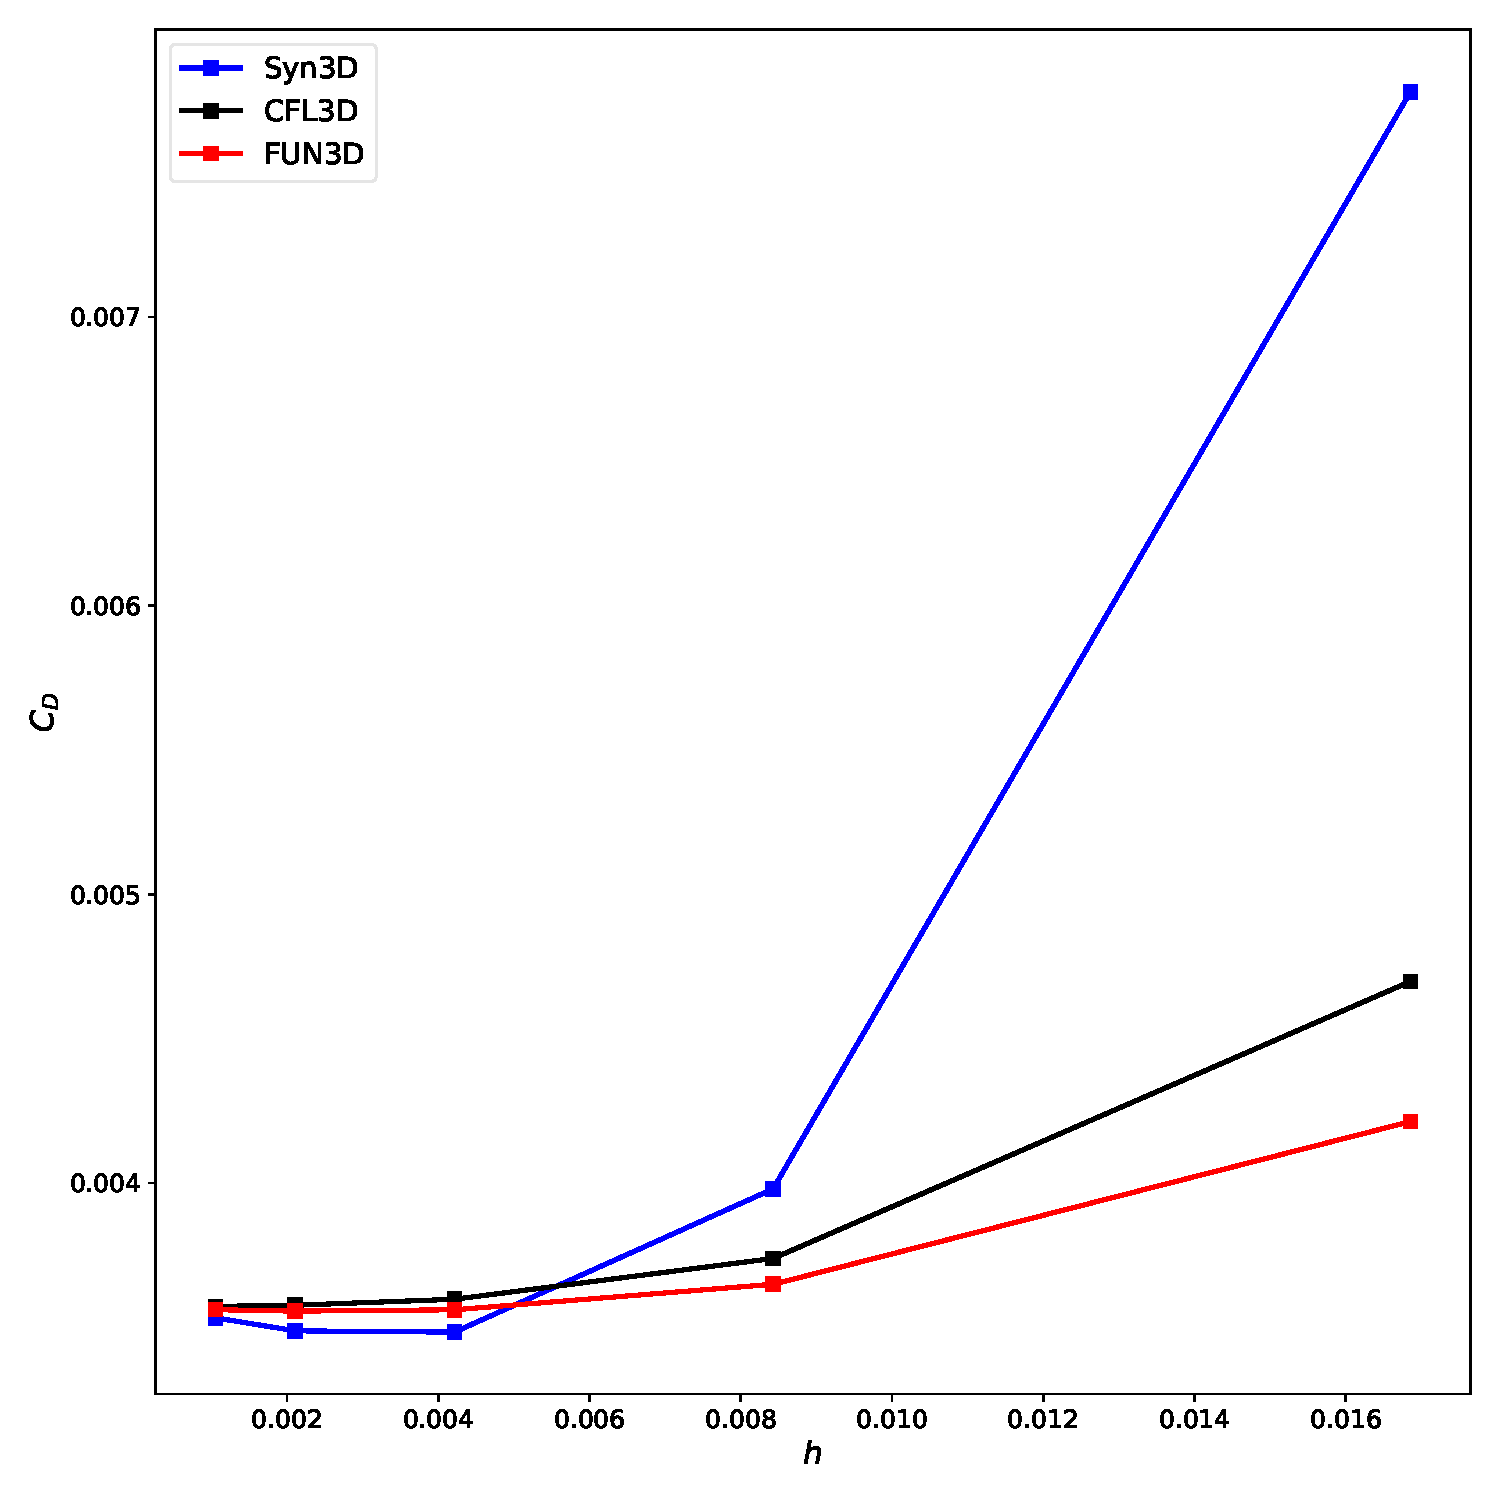
\includegraphics[width=1.0\textwidth]{figs/2dbump/C_DGridStudy.pdf}
  \caption{Drag coefficient.}
\end{subfigure}
\\
\begin{subfigure}{.45\textwidth}
  \centering
  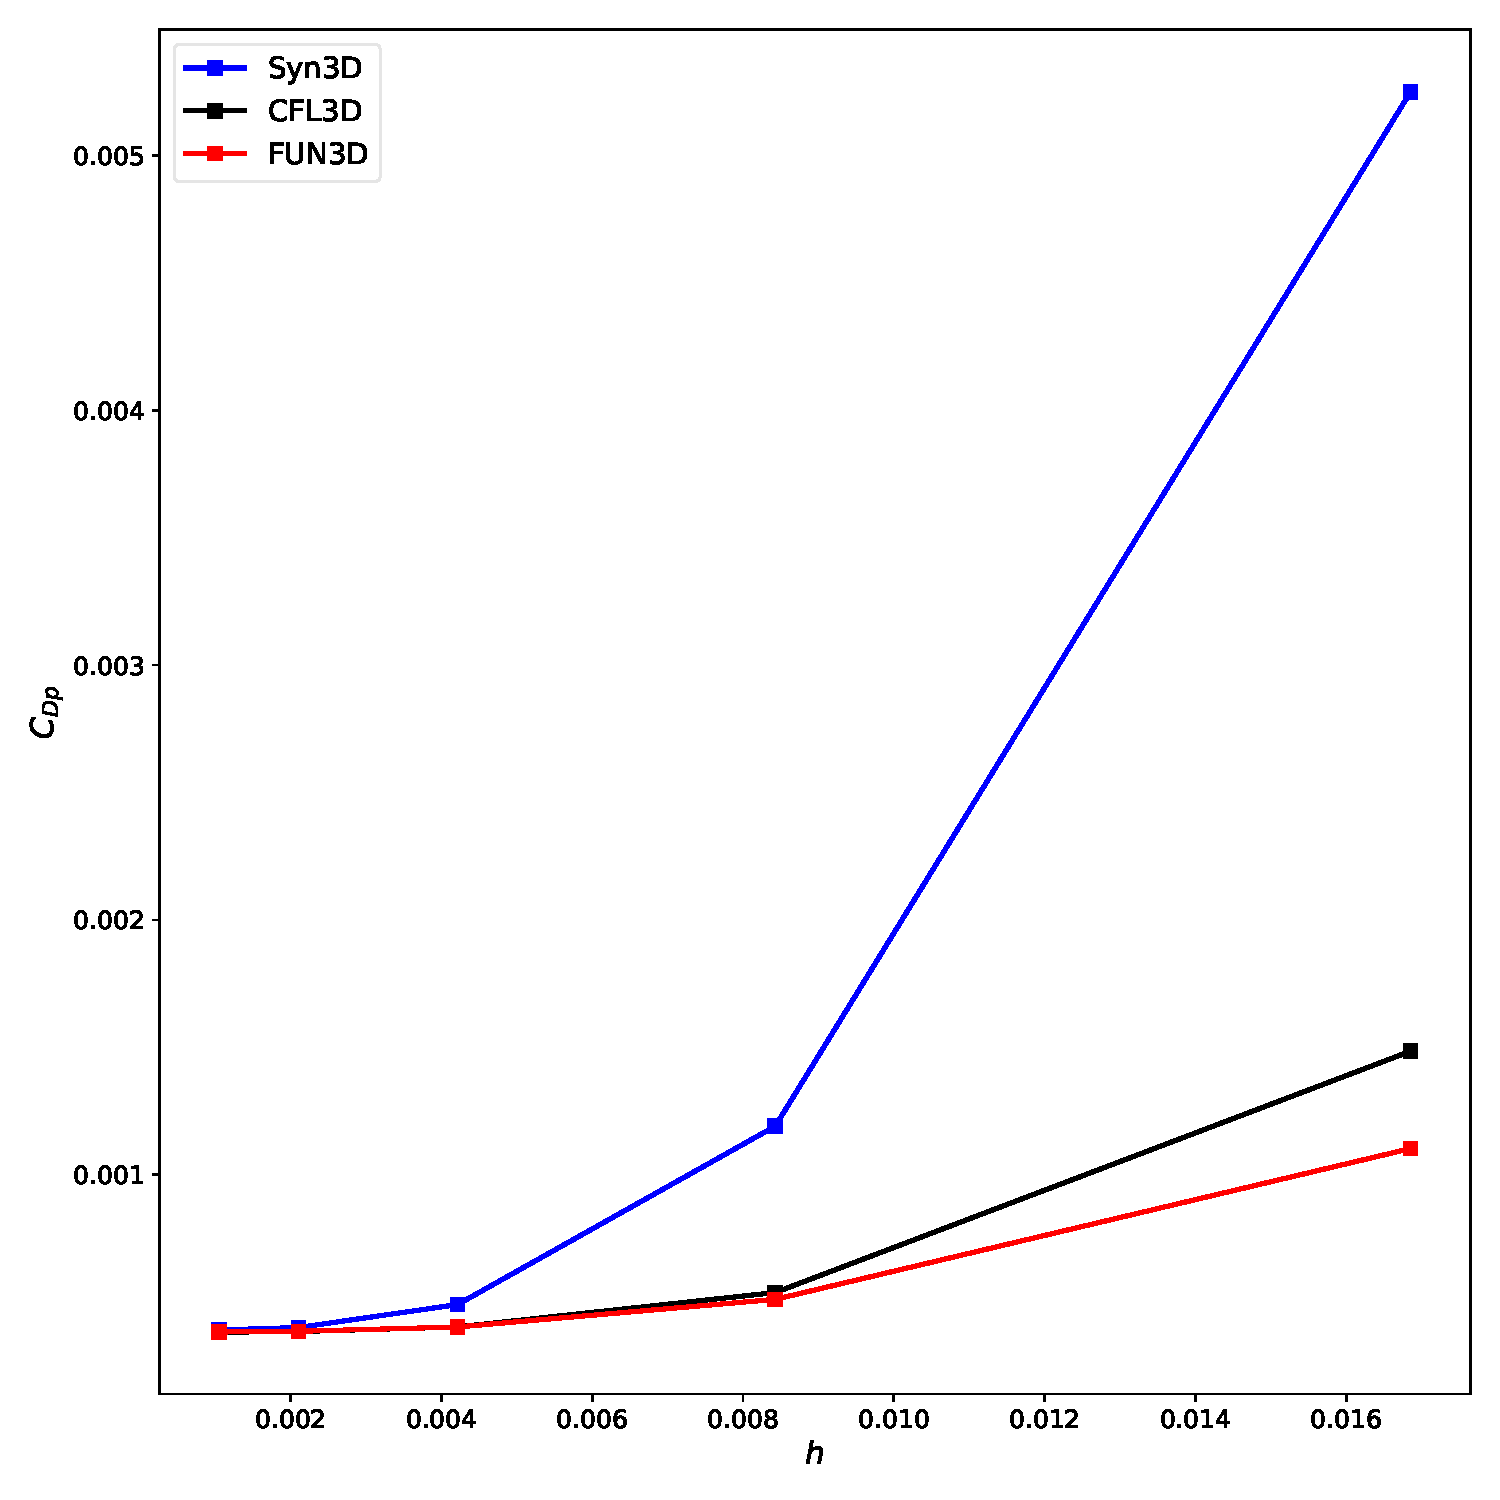
\includegraphics[width=1.0\textwidth]{figs/2dbump/C_DpGridStudy.pdf}
  \caption{Pressure contribution to drag.}
\end{subfigure}%
\begin{subfigure}{.45\textwidth}
  \centering
  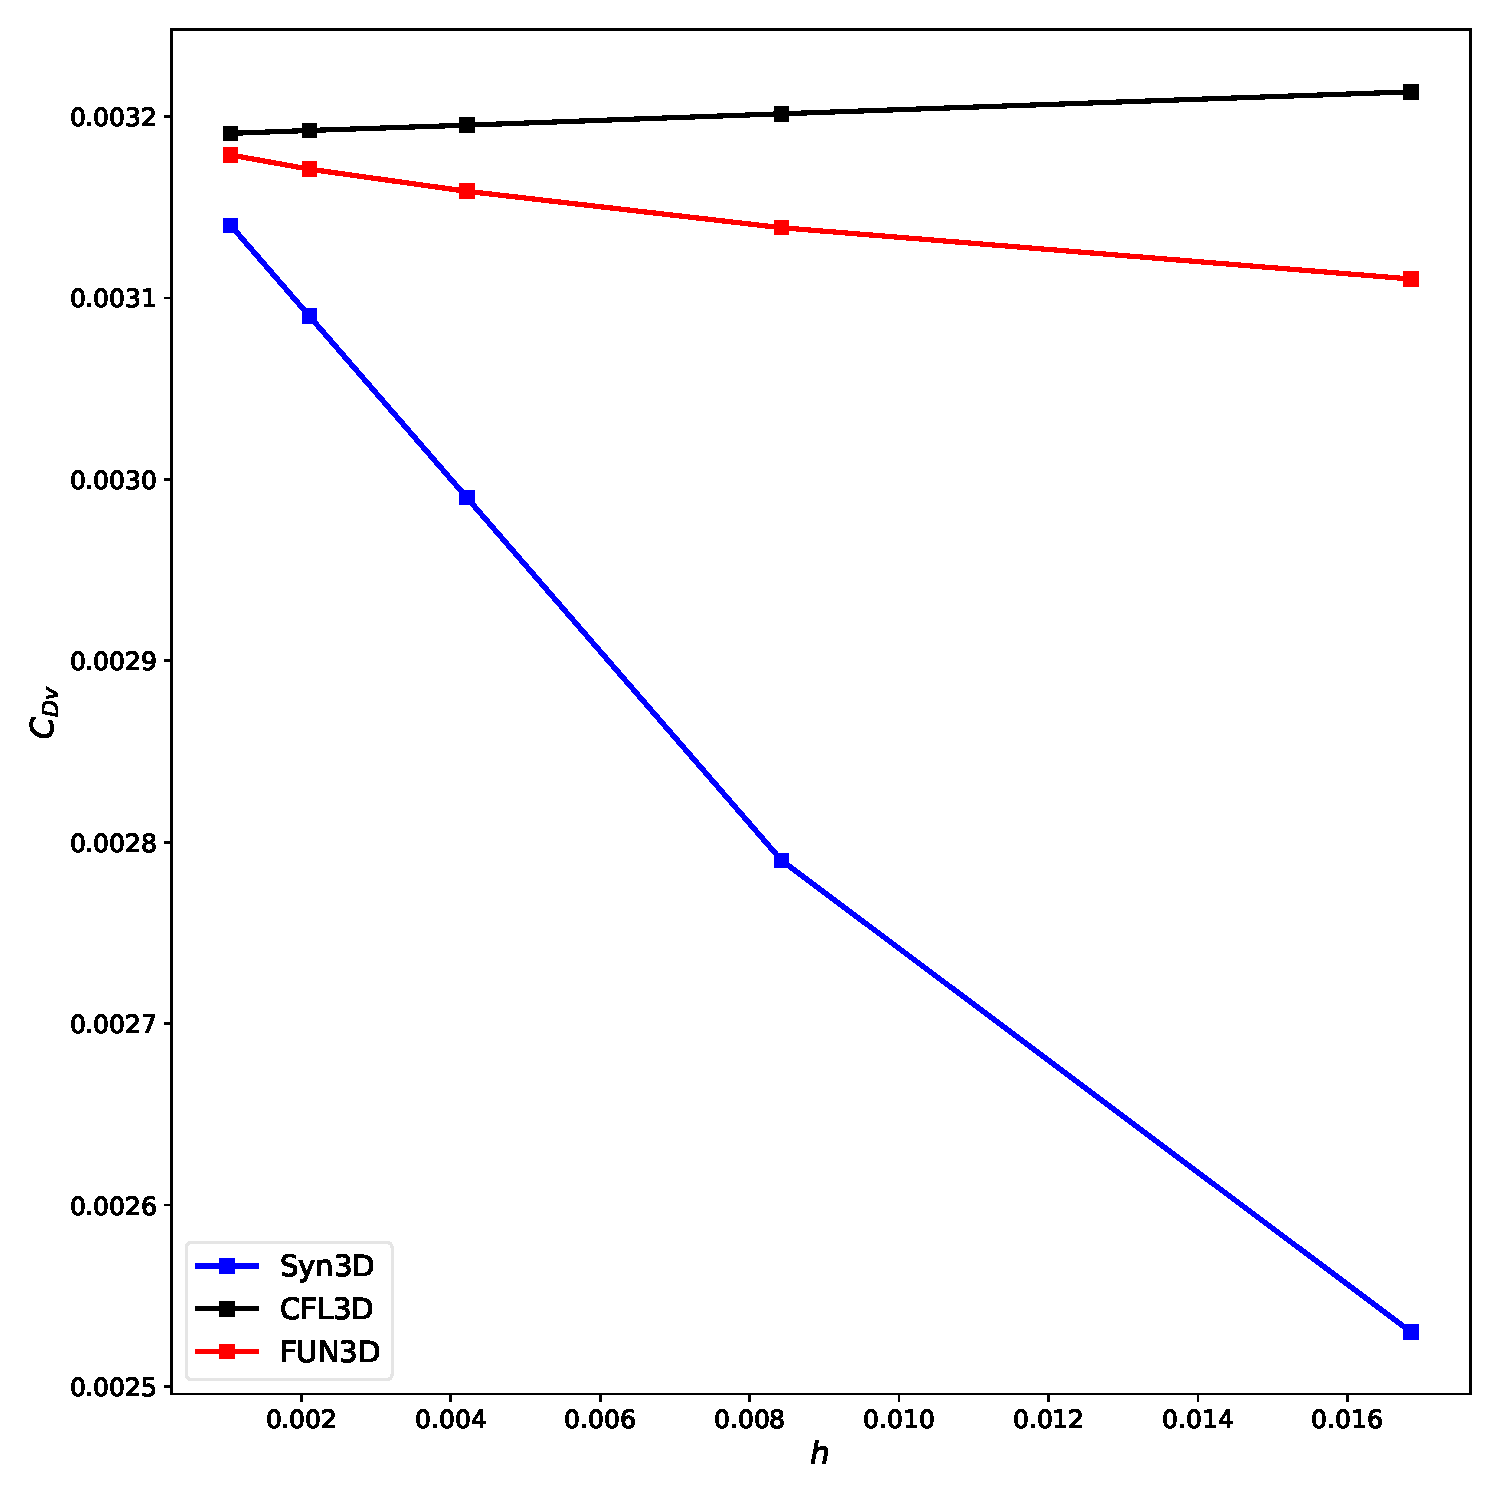
\includegraphics[width=1.0\textwidth]{figs/2dbump/C_DvGridStudy.pdf}
  \caption{Viscous contribution to drag.}
\end{subfigure}
\caption{2D Bump (syn3D): Force coefficients for various grid sizes.}
\label{fig:syn2dbumpforcestudy}
\end{figure}

\begin{figure}[ht!]
\centering
\begin{subfigure}{.45\textwidth}
  \centering
  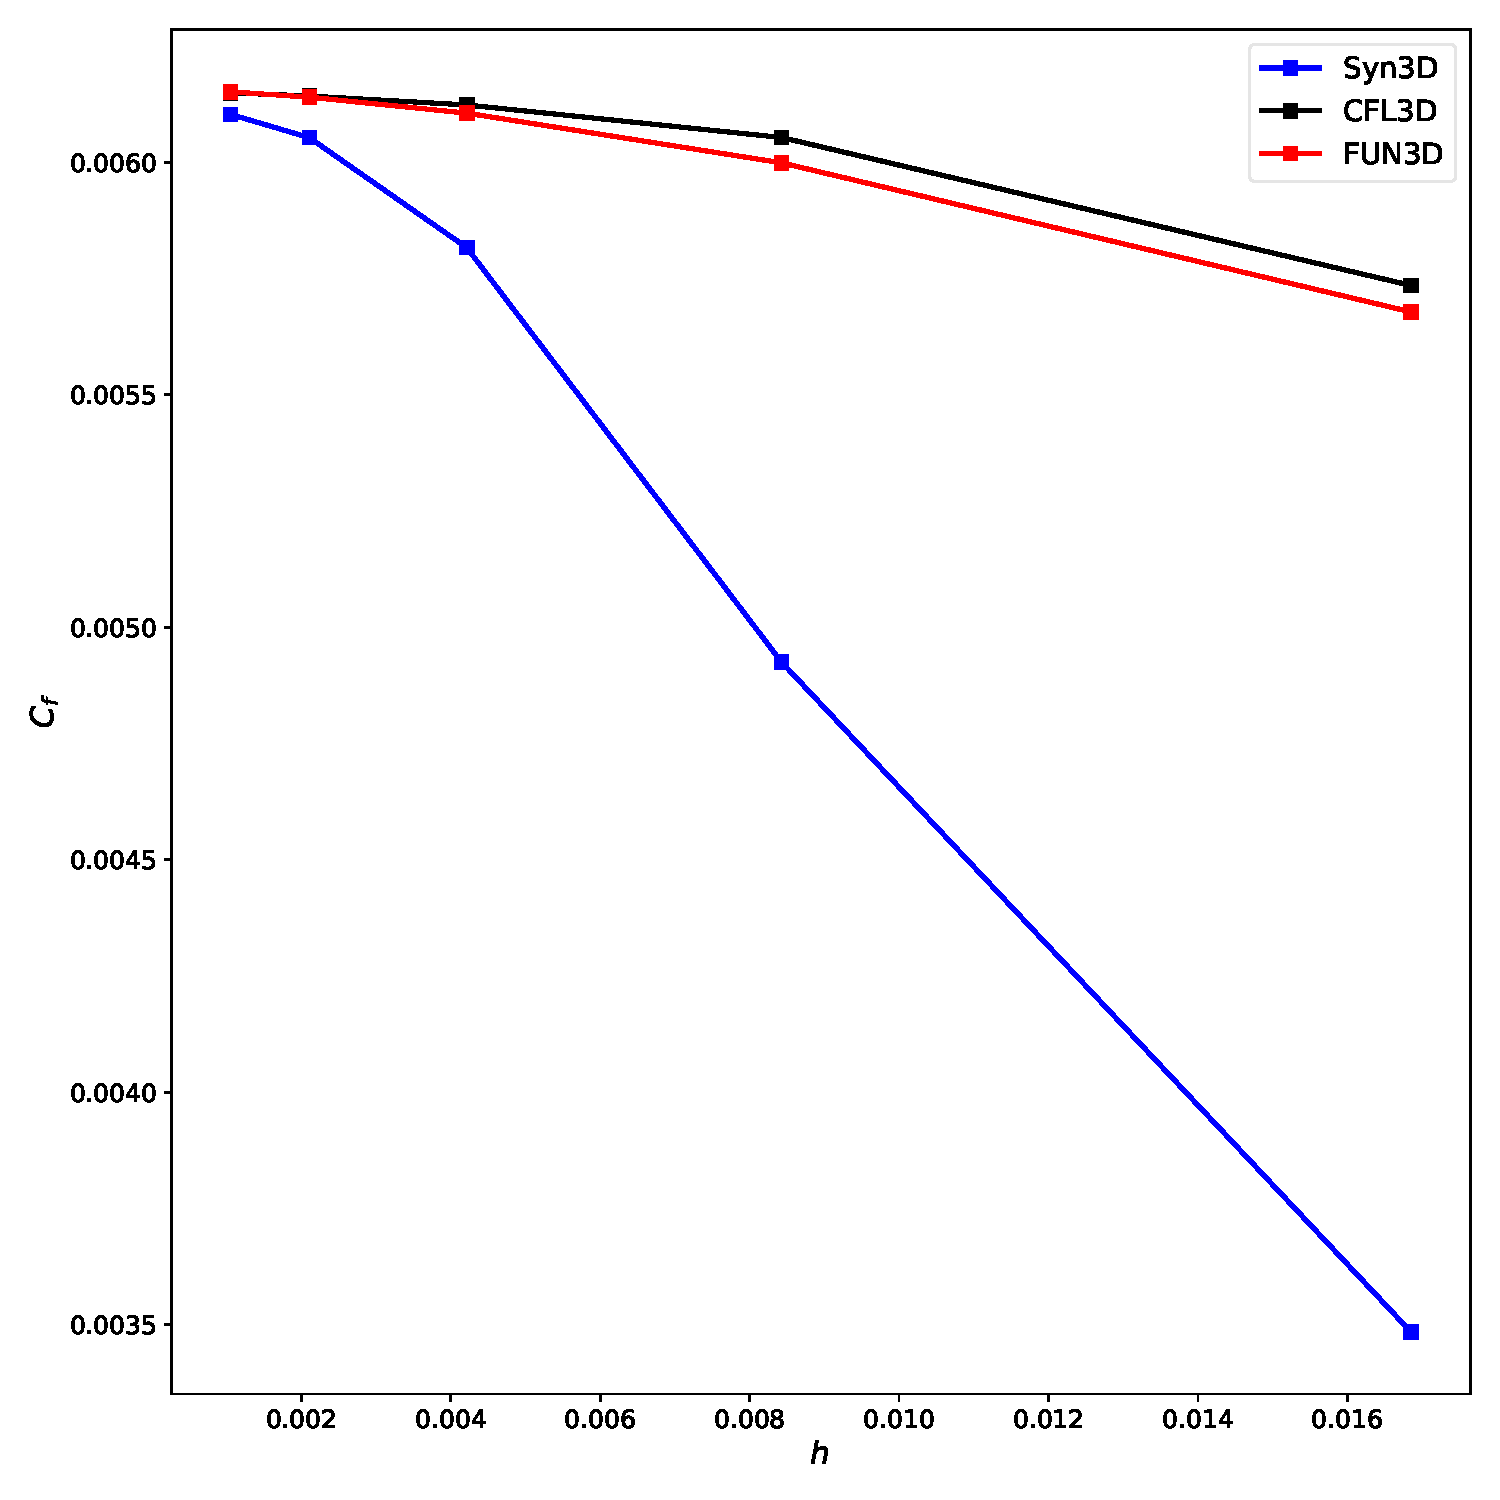
\includegraphics[width=1.0\textwidth]{figs/2dbump/Cf075GridStudy.pdf}
  \caption{$C_f$ grid study where x=0.75}
\end{subfigure}%
\begin{subfigure}{.45\textwidth}
  \centering
  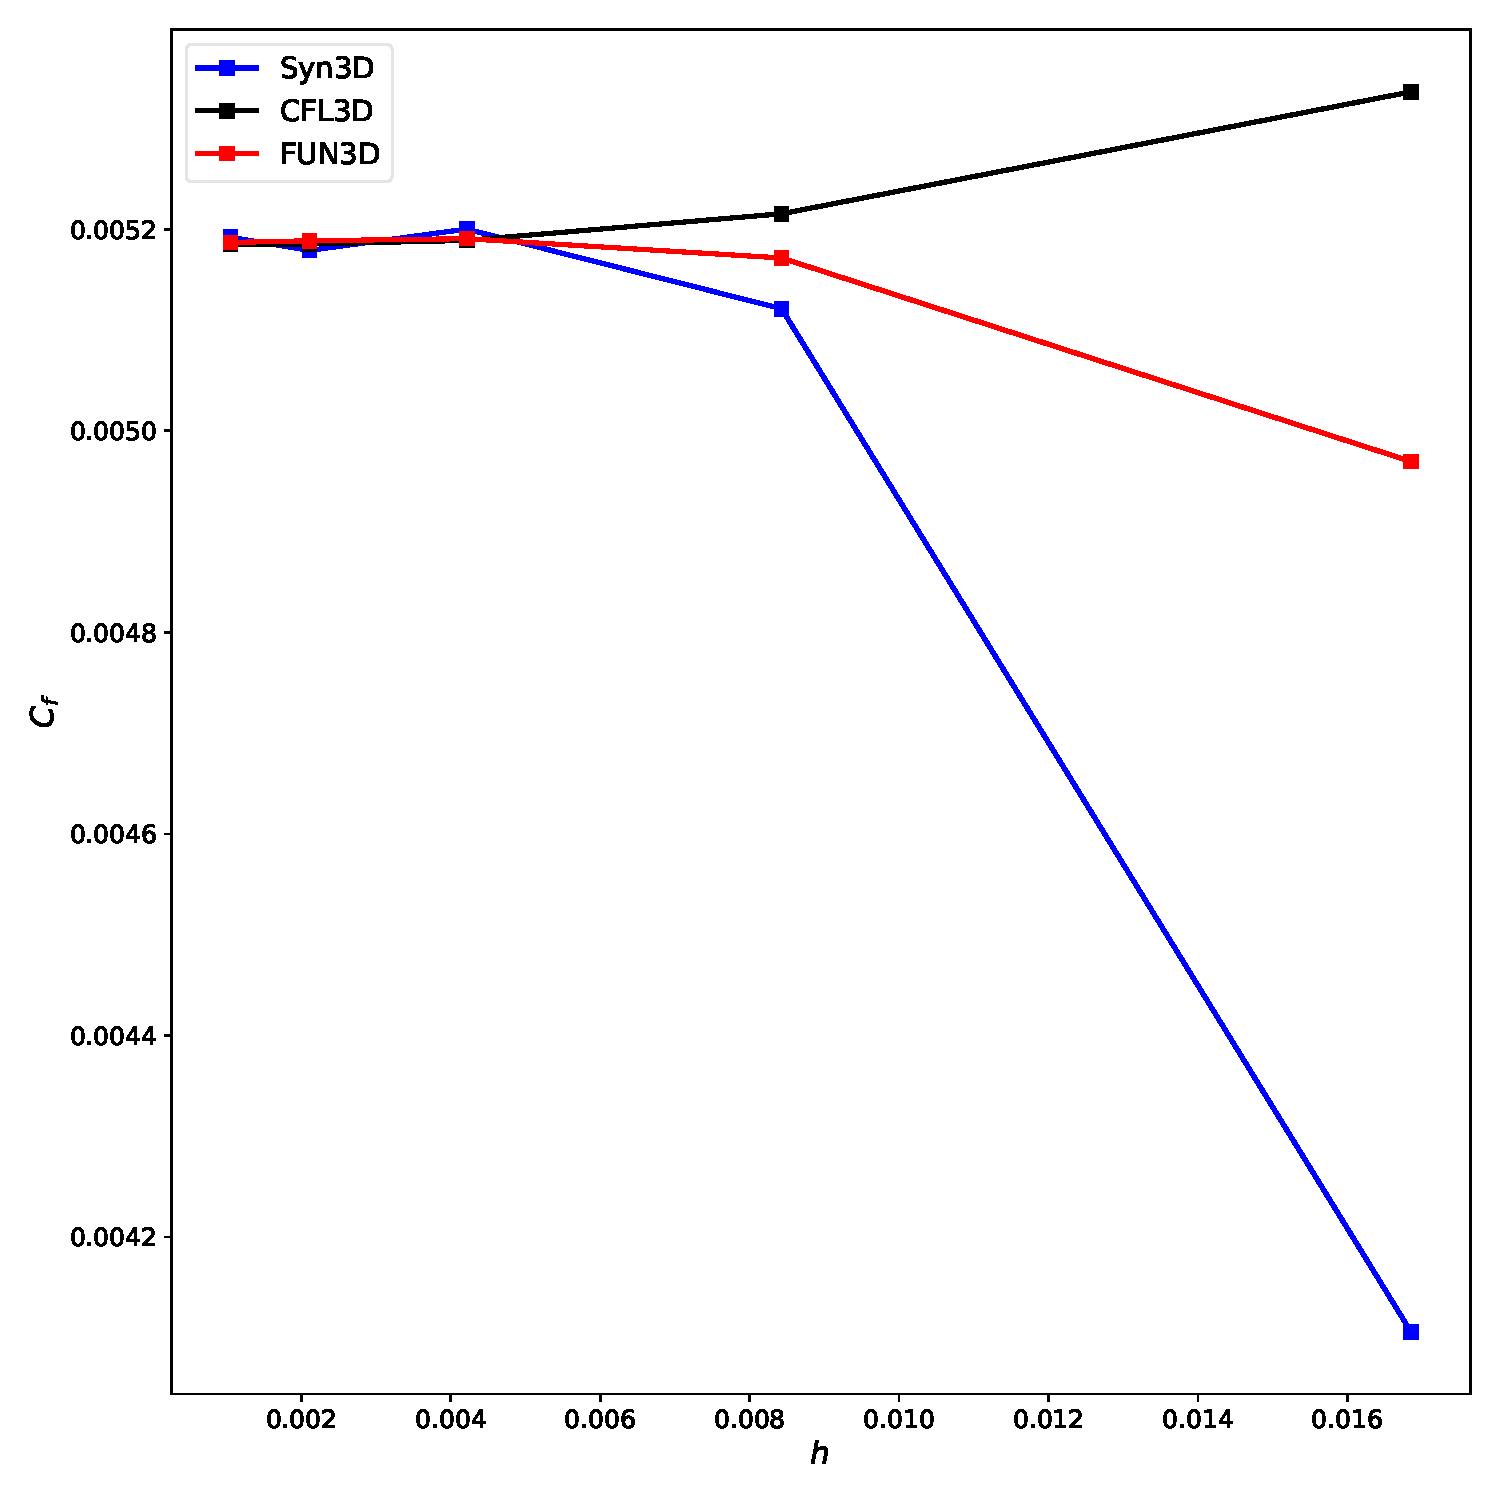
\includegraphics[width=1.0\textwidth]{figs/2dbump/Cf06321975GridStudy.pdf}
  \caption{$C_f$ grid study where x=0.6321975}
\end{subfigure}
\\
\begin{subfigure}{.45\textwidth}
  \centering
  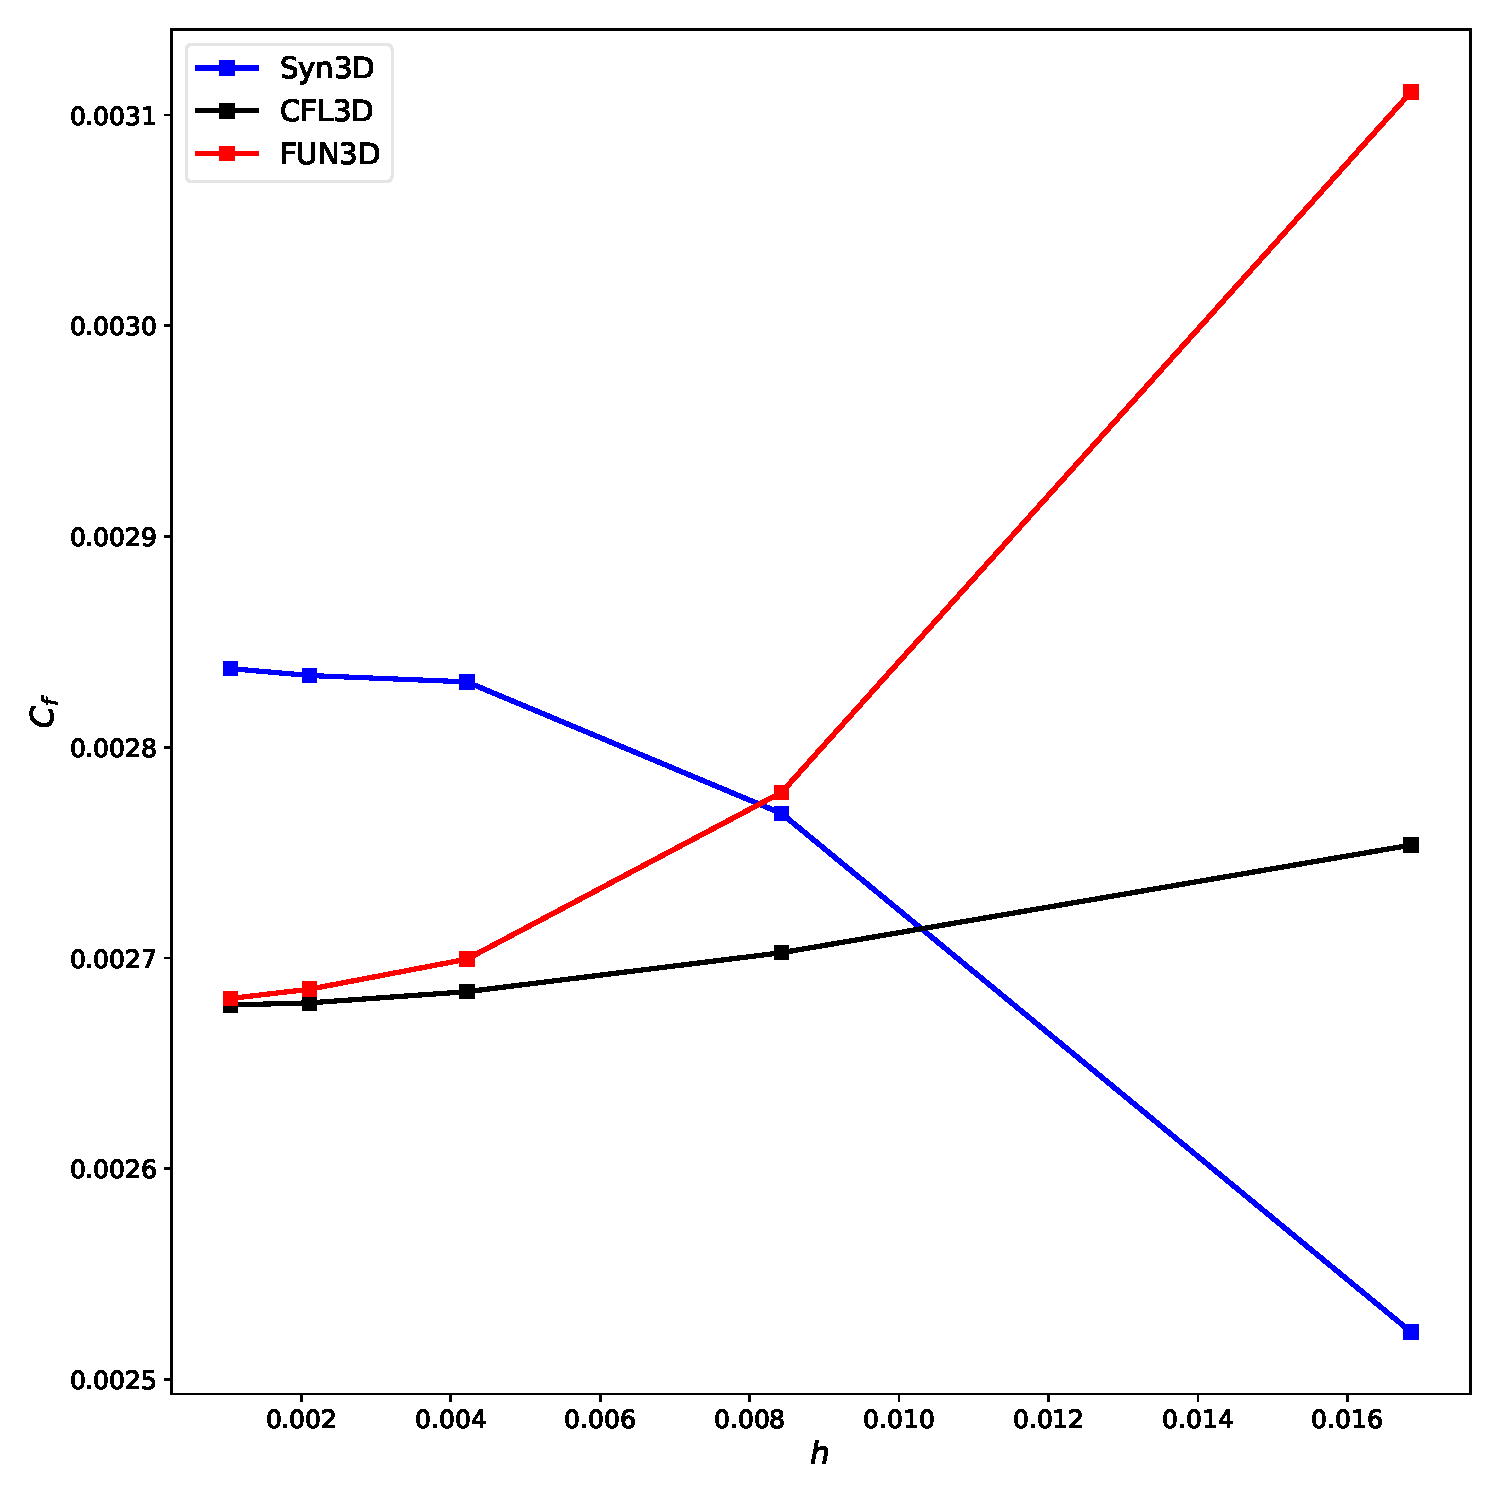
\includegraphics[width=1.0\textwidth]{figs/2dbump/Cf08678025GridStudy.pdf}
  \caption{$C_f$ grid study where x=0.8678025}
\end{subfigure}%}
\caption{2D Bump (syn3D): Skin friction coefficient at specific locations for various grid sizes.}
\label{fig:syn2dbumpcflocstudy}
\end{figure}

\Cref{fig:syn2dbumpcfstudy,fig:syn2dbumpcpstudy} show $C_f$ and $C_p$ distributions along the bump for all grids. Both plots show over-dissipated results for the coarser grids, which is expected, as discussed for the flat plate case. The difference of $C_f$ between the coarsest and finest grid is much greater than that of $C_p$. In other words, pressure seems to be less sensitive to mesh refinement than the skin friction. By the same token, while there is seemingly no difference of $C_p$ between the second finest and finest grids, indicating that grid convergence is achieved, there remains a noticeable discrepancy for $C_f$, which indicates its greater sensitivity to grid refinement.

\Cref{fig:syn2dbumpmutstudy} compares the eddy viscosity distribution between grids. The peak at the leading edge is significantly more pronounced for the coarser grids, and even slightly extends upstream. This results in over-predicted values for most, but not all, of the length of the wall; $\mu_t$ is under-predicted after $x\approx1.0$. Again, this is due to increased dissipation in the coarser grids, where the gradients are not as sharp as they should be.

\Cref{fig:syn2dbumpforcestudy,fig:syn2dbumpcflocstudy} show the convergence of force coefficients and skin friction for various grid sizes, compared with results from CFL3D and FUN3D. Again, it can be seen that there is much more dependence on grid size for syn3D as compared to the NASA solvers, although most values are very similar on the finest grid. The pressure contribution to drag, seems to have reached the asymptotic range of convergence, although the same cannot be said of the viscous contribution. Without a doubt, this increased dependence on grid size is due to the peak in eddy viscosity at the leading edge, which is an interface between block boundaries.
